\documentclass[preprint,12pt]{elsarticle}

\usepackage{amsmath}
\usepackage{amssymb}
\usepackage{hyperref}
\usepackage{booktabs}
\usepackage{multirow}
\usepackage{subcaption}
\usepackage{xcolor}
\usepackage{colortbl}
\usepackage{float}

\begin{document}

\begin{frontmatter}

\title{patX: Interpretable Pattern Extraction for Time Series and Spatial Data}

\author{Joshua Wolber}
\affiliation{organization={}}

\begin{abstract}
We introduce \textbf{patX}, an open--source Python package that bridges the gap
between the automatic pattern learning capabilities of convolutional neural
networks (CNNs) and the interpretability requirements of biomedical applications.
Like CNNs, patX automatically discovers discriminative patterns from input data
and uses them for prediction; however, unlike CNNs where learned patterns remain
opaque, patX makes this pattern learning explicit and interpretable through
human--readable B--spline templates.
By framing pattern discovery as a constrained optimization problem over
B--spline templates across multiple signal transformations (e.g. raw, wavelet, FFT,
derivative), patX learns compact, highly predictive patterns that serve as
transparent input features for conventional machine--learning models.
patX also supports spatially or temporally invariant pattern detection.
By default, it evaluates a learned template in a sliding window over an allowed
range and uses the best match (minimum RMSE) as the feature value.
This is analogous to applying a convolutional filter across positions followed
by global pooling, yielding translation invariance.
If sliding is disabled, each pattern is evaluated at a single index, producing
position-specific features.

We evaluate patX on seven diverse biomedical tasks: (i) glucose forecasting
(AZT1D), (ii) arrhythmia classification (MITBIH), (iii) emotion classification
from EEG signals (Emotions), (iv) gene expression prediction from epigenetic
signatures (REMC), (v) acute respiratory distress syndrome (ARDS)
classification in an intensive care unit (MIMIC--IV), (vi) human activity
recognition from inertial measurement unit (IMU) sensors (PAMAP2), and (vii)
voice pathology detection (SVD).
We compare against standard automated feature extraction baselines and a CNN
baseline under matched splits and metrics.

Beyond predictive performance, patX's interpretable pattern discovery can lead
to novel scientific insights: from histone modification data, it can reveal
which modifications are most informative at specific genomic positions; from
ECG data, spectral features may uncover potential electrophysiological causes
of arrhythmias; and from glucose data, different temporal patterns can reveal
the relative importance of short-term versus long-term dynamics for different
patient populations.
This transparent approach to automatic feature extraction addresses the
``black box'' criticism of deep learning while maintaining competitive
performance, making patX particularly suitable for clinical applications where
explainability is crucial.
Our tool is available at \url{https://github.com/Prgrmmrjns/patX} and offers a
simple interface for extracting interpretable patterns from time series and
spatial data.
\end{abstract}

%%Graphical abstract
\begin{graphicalabstract}
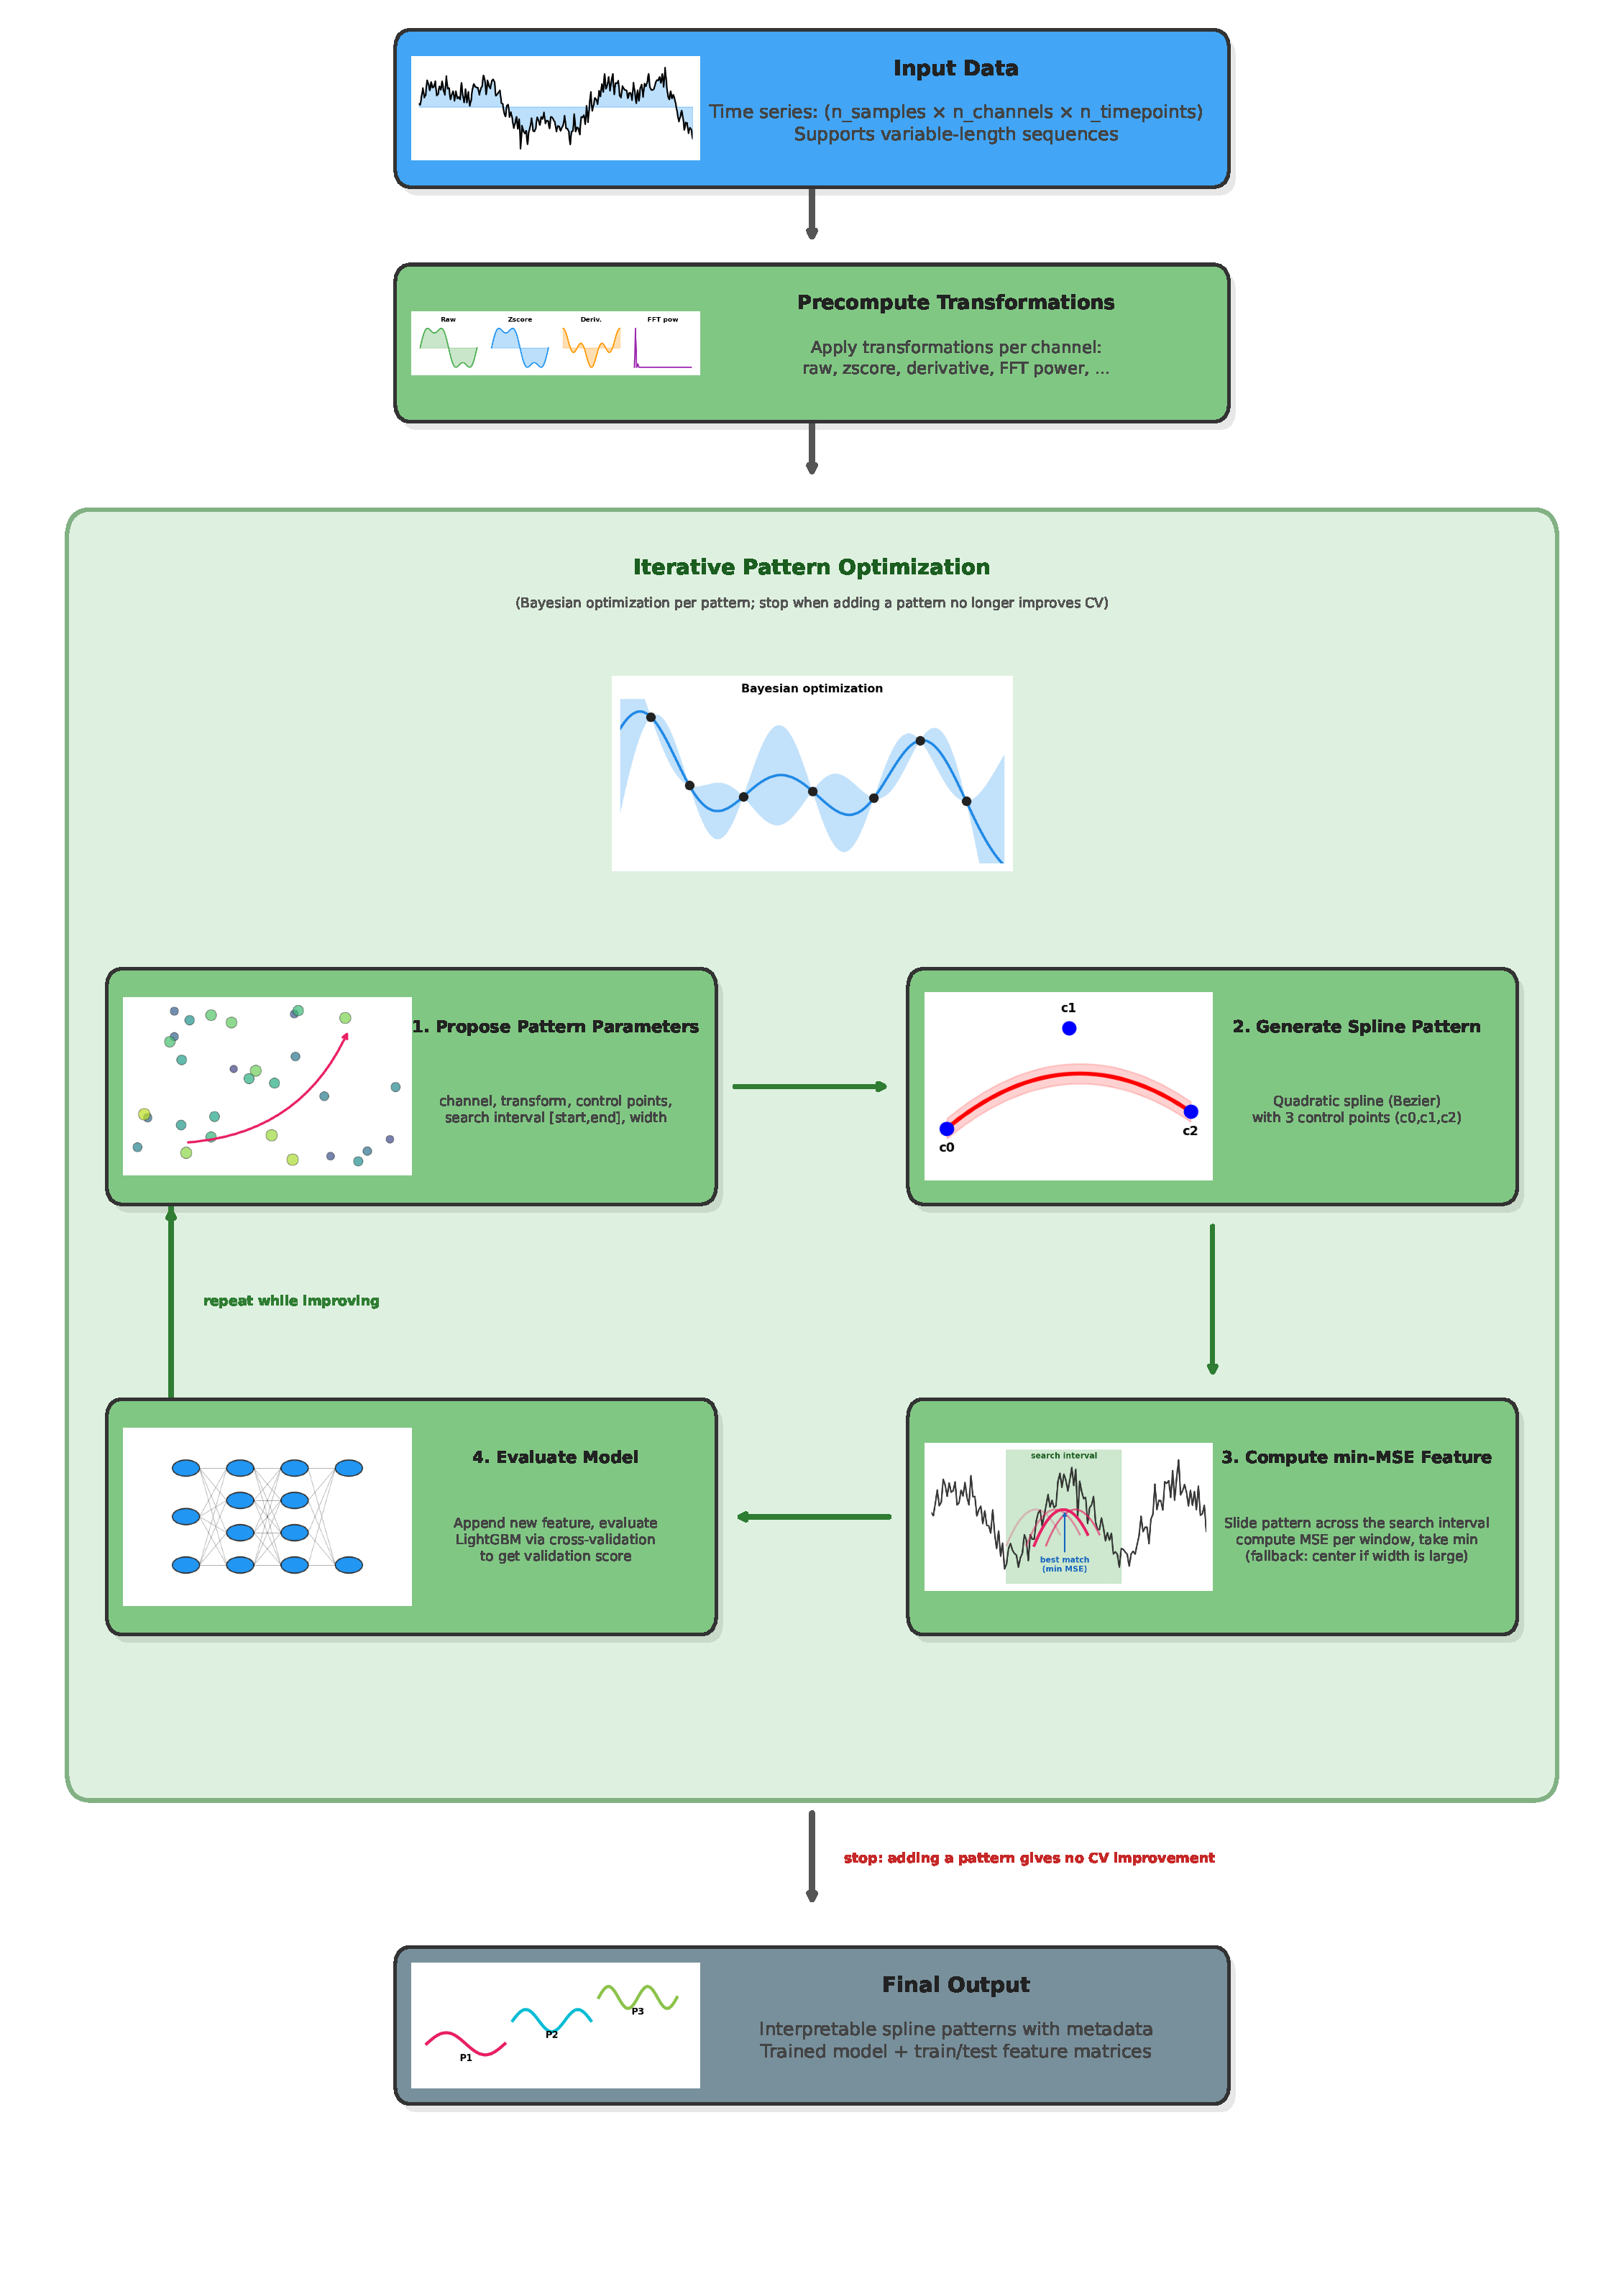
\includegraphics[width=\textwidth]{images/flowchart/flowchart.pdf}
\end{graphicalabstract}

\begin{highlights}
\item patX learns interpretable B-spline templates as explicit features.
\item patX is best on 6 of 7 biomedical benchmarks under matched protocols.
\item Ablations show shifting and search budget are dataset-dependent knobs.
\end{highlights}

\begin{keyword}
interpretable machine learning \sep time series \sep pattern discovery \sep
B-splines \sep feature extraction
\end{keyword}

\end{frontmatter}

\section{Introduction}
Biomedical research has witnessed an unprecedented expansion in the
generation and utilization of high-resolution time series and spatial data
across multiple domains.
From continuous physiological monitoring through electrocardiography (ECG)
and electroencephalography (EEG) to advanced spatially-resolved omics
technologies, these data modalities have become fundamental to modern
healthcare and biomedical discovery \cite{morid2023time, rood2022impact}.

Time series data in healthcare captures the temporal evolution of patient
health, offering crucial insights into disease progression, treatment
effectiveness, and physiological dynamics \cite{patharkar2024predictive}.
Continuous monitoring systems generate vast streams of physiological
signals---from ECG and EEG to glucose monitoring---that contain rich information
about both normal physiology and pathological states
\cite{chaddad2023electroencephalography, anbalagan2023analysis}.
In genomics, spatial profiling of chromatin modifications provides insights into
regulatory mechanisms underlying development and disease \cite{yadav2022systems}.

The analysis of biomedical time series and spatial data has evolved through
three different paradigms that represent fundamentally different philosophies
toward feature representation and model development.
Traditional approaches to biomedical signal analysis rely heavily on domain
expertise to manually craft features capturing relevant temporal and spatial
characteristics \cite{fulcher2018feature}.
For ECG analysis, features include heart rate variability and QRS complex
morphology \cite{gelen2025novel, ansari2023deep}; for EEG, frequency band power
and coherence measures \cite{moutonnet2025augmentation}.
While providing clear physiological interpretations, this approach is
labor-intensive, requires extensive domain expertise, and may miss subtle
patterns in complex datasets \cite{miotto2018deep,ansari2023deep}.

Comprehensive automated feature extraction libraries address scalability by
systematically computing large feature sets.
tsfresh extracts up to 1,558 features \cite{christ2018tsfresh}, while catch22
provides 22 carefully selected features optimized for performance and efficiency
\cite{lubba2019catch22}.
While effective at uncovering patterns, these libraries introduce challenges
related to interpretability and feature selection from high-dimensional spaces
\cite{henderson2021empirical, petelin2023towards}.

Deep learning methods learn hierarchical feature representations directly from
raw data through end-to-end training \cite{miotto2018deep}.
CNNs automatically learn temporal patterns through convolutional filters
\cite{wang2022systematic}, while RNNs and LSTMs model sequential dependencies
\cite{lee2021modeling}.
However, these approaches face significant interpretability challenges, creating
barriers to clinical adoption where explainability is crucial
\cite{rudin2019stop, ennab2024enhancing}.

This evolution reflects a fundamental trade-off between interpretability and
automated pattern discovery: manual approaches offer interpretability but lack
scalability, automated libraries provide scalability but reduce interpretability,
and deep learning offers performance but sacrifices explainability.

B-splines provide smooth curve representations with local control, where
adjusting one control point affects only a bounded region
\cite{balestriero2018spline}.
Recent work shows deep networks with piecewise-linear activations implicitly
construct spline-based templates through gradient descent, but these
representations remain opaque \cite{balestriero2018spline}.
This connection suggests directly optimizing interpretable B-spline patterns as
explicit templates, bypassing deep learning's black-box nature while retaining
spline-based representational power.

Pattern-based approaches identify characteristic subsequences and measure
similarity to query signals, connecting to matched filtering in signal
processing theory.
The key challenge is discovering templates automatically: manual specification
requires expertise, exhaustive search is prohibitive, and recent deep learning
approaches sacrifice interpretability.
An effective method must balance automatic discovery, computational efficiency,
and interpretability, while capturing both shape and amplitude information.

We address the fundamental trade-off between automation, performance, and
interpretability with \textbf{patX}, a method that combines spline-based
pattern representations with evolutionary optimization for automatic template
discovery.
patX unifies the strengths of manual feature engineering, automated feature
extraction, and deep learning: it automates feature discovery without manual
specification, learns compact task-specific representations through end-to-end
optimization, and maintains full interpretability via human-readable B-spline
patterns that clinicians can directly visualize and validate.

A key innovation of patX is its multi-representation search strategy.
Rather than operating solely on raw signals, patX precomputes multiple signal
transformations---including wavelet decompositions, Fourier transforms, and
derivatives---and automatically selects the most discriminative representation
for each pattern during optimization.
This allows patterns to match signals in the time domain, frequency domain,
or derivative space, capturing diverse signal characteristics that would
require manual specification in traditional feature engineering approaches.

patX searches over start positions, widths, channels, B-spline control
points, temporal shifts, pattern scaling modes (absolute vs. relative), and
signal transformations to automatically learn discriminative patterns.
Each discovered pattern induces a dissimilarity feature measuring the root mean
squared error (RMSE) between the pattern template and the corresponding
transformed signal segment, with temporal shifts allowing for robust matching
of misaligned patterns.
The optimization process also determines whether to match a pattern's absolute
values---capturing both shape and amplitude---or its relative shape, enabling
patX to distinguish between a wider range of morphological characteristics.

We evaluate patX across seven heterogeneous biomedical problems: arrhythmia
classification on MIT-BIH \cite{MoodyMark1992,Goldberger2000}, emotion
classification from EEG signals (Emotions), gene expression prediction
from histone modification profiles (REMC) \cite{Roadmap2015}, clinical
prediction on MIMIC-IV \cite{Johnson2023MIMICIV} (ARDS classification),
glucose forecasting (AZT1D), human activity recognition from IMU sensors
(PAMAP2) \cite{Reiss2012PAMAP2}.
We compare against tsfresh \cite{christ2018tsfresh}, catch22 \cite{lubba2019catch22}, 
and a convolutional neural network baseline under matched splits and metrics.

We introduce patX, a B-spline-based pattern discovery method that
produces human-readable motifs bridging spline theory and template matching
for interpretable time series analysis, with automatic selection of signal
representations across multiple transformations (time, frequency, derivative).
We evaluate patX against established baselines on seven diverse biomedical
datasets under matched splits and metrics, and analyze the learned patterns for
interpretability and domain relevance.
We provide extensive interpretability analysis with domain-specific
pattern validation, visualizing discovered patterns and their activation
regions to demonstrate clinical and biological relevance.
We release patX as an official Python package on PyPI:
(\url{https://pypi.org/project/patx/}).

\section{Related Work}

Machine learning approaches for the biomedical tasks we address have evolved
from classical methods to specialized deep architectures achieving impressive
performance on individual benchmarks.
We review state-of-the-art methods for each domain, highlighting methodological
differences to contextualize patX's positioning as a general-purpose
interpretable framework.

\textbf{ECG arrhythmia classification.}
Deep learning has dramatically advanced ECG analysis.
Hannun et al.\ achieved cardiologist-level performance using a 34-layer
residual CNN trained on over 90,000 single-lead ECGs \cite{hannun2019cardiologist}.
Acharya et al.\ introduced deep CNN architectures specifically optimized for
MIT-BIH heartbeat classification, achieving 94--99\% accuracy
\cite{acharya2017deep, ansari2023deep}.
Sannino and De Pietro achieved 99.3\% accuracy using an 11-layer CNN with
intra-patient evaluation, where beats from the same patient appear in both
training and test sets \cite{sannino2018deep}.
Hybrid CNN-LSTM models reach 99.5\% accuracy by combining spatial and
temporal feature learning \cite{liu2022arrhythmia}.
Critically, most high-performing methods use \textit{intra-patient} evaluation
protocols with abundant training data; inter-patient evaluation (as we employ)
is substantially more challenging and clinically relevant.

\textbf{Glucose forecasting.}
Blood glucose prediction has been extensively studied using recurrent
architectures.
Li et al.\ developed convolutional-recurrent networks achieving 10--14 mg/dL
RMSE for 30-minute prediction horizons \cite{li2020glucose}.
Xie and Wang benchmarked multiple ML algorithms on Type 1 diabetes data,
finding that LSTM and random forest achieve 15--20 mg/dL RMSE depending on
prediction horizon and preprocessing \cite{xie2020benchmarking}.
Van Doorn et al.\ incorporated physical activity data alongside CGM,
achieving 19.5 mg/dL RMSE \cite{van2021machine}.
These approaches typically require patient-specific fine-tuning and careful
handling of insulin/carbohydrate covariates through domain-specific
preprocessing \cite{woldaregay2019data}.
patX provides an interpretable alternative by learning explicit templates that
can capture glucose dynamics without manual motif specification.

\textbf{Gene expression prediction from epigenomics.}
DeepChrome pioneered deep learning for predicting gene expression from histone
modifications, using CNNs to learn combinatorial patterns across 100 bins
around transcription start sites \cite{singh2020deep}.
DeepDiff extended this to predict differential expression between cell types
\cite{sekhon2018deepdiff}.
Frasca et al.\ demonstrated that interpretable linear models on well-chosen
histone features can match deep learning performance while providing biological
insights \cite{frasca2022interpretable}.
Our prior work PatternChrome used particle swarm optimization to discover
interpretable histone patterns \cite{paul2025prediction}.
PatX differs by discovering patterns through B-spline optimization rather than
fixed bin aggregation, enabling flexible pattern positioning and shape learning.

\textbf{Human activity recognition.}
IMU-based activity recognition benefits from deep temporal modeling.
Ord{\'o}{\~n}ez and Roggen combined CNNs with LSTMs for multimodal wearable
data, achieving strong performance on PAMAP2 \cite{ordoez2016deep}.
Tan et al.\ introduced CNN with multihead attention, achieving 98\%+ accuracy
through learned temporal attention weights \cite{tan2023cnn}.
Hammerla et al.\ systematically compared deep architectures, finding that
bidirectional LSTMs excel at capturing long-range dependencies
\cite{hammerla2016deep}.
Recent state-space models (HARMamba) report F1 scores exceeding 99\% through
selective state modeling \cite{bollampally2024optimizing}.
These methods use leave-one-subject-out or similar protocols;
patX provides an interpretable alternative by representing motifs as explicit
templates and turning template matches into transparent features.

\textbf{Clinical outcome prediction.}
ARDS prediction from ICU time series has been addressed using gradient boosting
and deep learning.
Villar et al.\ developed ML models achieving 0.87 AUC for ICU mortality
prediction in moderate-to-severe ARDS patients using carefully selected
clinical features \cite{villar2023predicting}.
Le et al.\ trained models for early ARDS prediction, achieving 0.80--0.85 AUC
with features derived from vital signs and laboratory values
\cite{le2020supervised}.
These approaches require extensive clinical feature engineering and
imputation strategies for irregular time series \cite{zhang2021ards}.
PatX provides an alternative approach using pattern-based features directly
on time series without manual feature specification.

\textbf{Voice pathology detection.}
Voice disorder classification using the Saarbr\"ucken Voice Database (SVD) has
been approached with various methods.
Mart{\'\i}nez et al.\ used GMM classifiers with MFCC, HNR, and glottal features,
achieving competitive results through 12-fold cross-validation and multi-vowel
fusion \cite{martinez2012voice}.
Huckvale and Buciuleac systematically analyzed evaluation protocols on SVD,
showing that performance varies significantly based on pathology subset and
audio materials used \cite{huckvale2021automated}.
Verde et al.\ compared SVM, random forest, and neural networks using 10-fold CV,
achieving 83--87\% accuracy \cite{verde2018voice}.
Deep CNN approaches on spectrograms achieve up to 95\% accuracy
\cite{muhammad2018pathological}, though evaluation protocols and pathology
subsets differ across studies \cite{islam2022voice, bhattacharjee2022voice}.

\textbf{EEG emotion classification.}
EEG-based emotion recognition has advanced through deep architectures.
Zhang et al.\ compared CNN, LSTM, and hybrid models, finding that CNN-LSTM
combinations achieve 90--95\% accuracy on DEAP and SEED datasets
\cite{zhang2020investigation}.
Islam et al.\ reviewed deep and shallow learning approaches, noting that
performance varies significantly based on feature extraction and electrode
selection \cite{islam2021emotion}.
Transformer-based models achieve 96--98\% on standard benchmarks through
learned attention over spatial and temporal EEG features.
patX offers a complementary approach: explicit, human-readable motifs that can
be inspected and related to known EEG structure (e.g., band-specific changes).

\textbf{Positioning of patX.}
These domain-specific methods achieve impressive performance through
task-tailored architectures, specialized preprocessing, and extensive
hyperparameter tuning.
Key methodological differences include: (1) \textit{evaluation protocols}---many
studies use intra-patient splits or high-fold CV providing more training data;
(2) \textit{architecture tuning}---specialized models require task-specific
layer configurations; (3) \textit{feature engineering}---clinical and voice
applications often require domain expert features.
In contrast, patX applies an identical pipeline across all seven tasks without
architecture modification, achieving competitive performance while providing
full interpretability through explicit B-spline patterns.
Rather than competing with specialized state-of-the-art systems, patX offers
a flexible, interpretable baseline that practitioners can customize through
user-defined transforms, ML models, and pattern configurations.

\section{Methods}

\subsection{Overview}
patX discovers interpretable patterns from time series and spatial data through
a four-stage pipeline: (1) signal transformation, (2) transform selection,
(3) pattern optimization, and (4) pattern refinement.
The core idea is simple: learn B-spline templates that represent characteristic
shapes in the data, then measure how well each signal matches these templates
using root mean squared error (RMSE).
These RMSE values become features for prediction.

The key insight is that discriminative patterns---shapes that differ
systematically between classes or correlate with outcomes---will produce RMSE
features that separate samples effectively.
By searching for patterns across multiple signal representations (raw signals,
derivatives, frequency spectra, wavelets), patX can discover features in
whichever domain is most informative for a given task.

An overview of the patX methodology is shown in Figure~\ref{fig:patx_methodology}.

\begin{figure}[H]
  \centering
  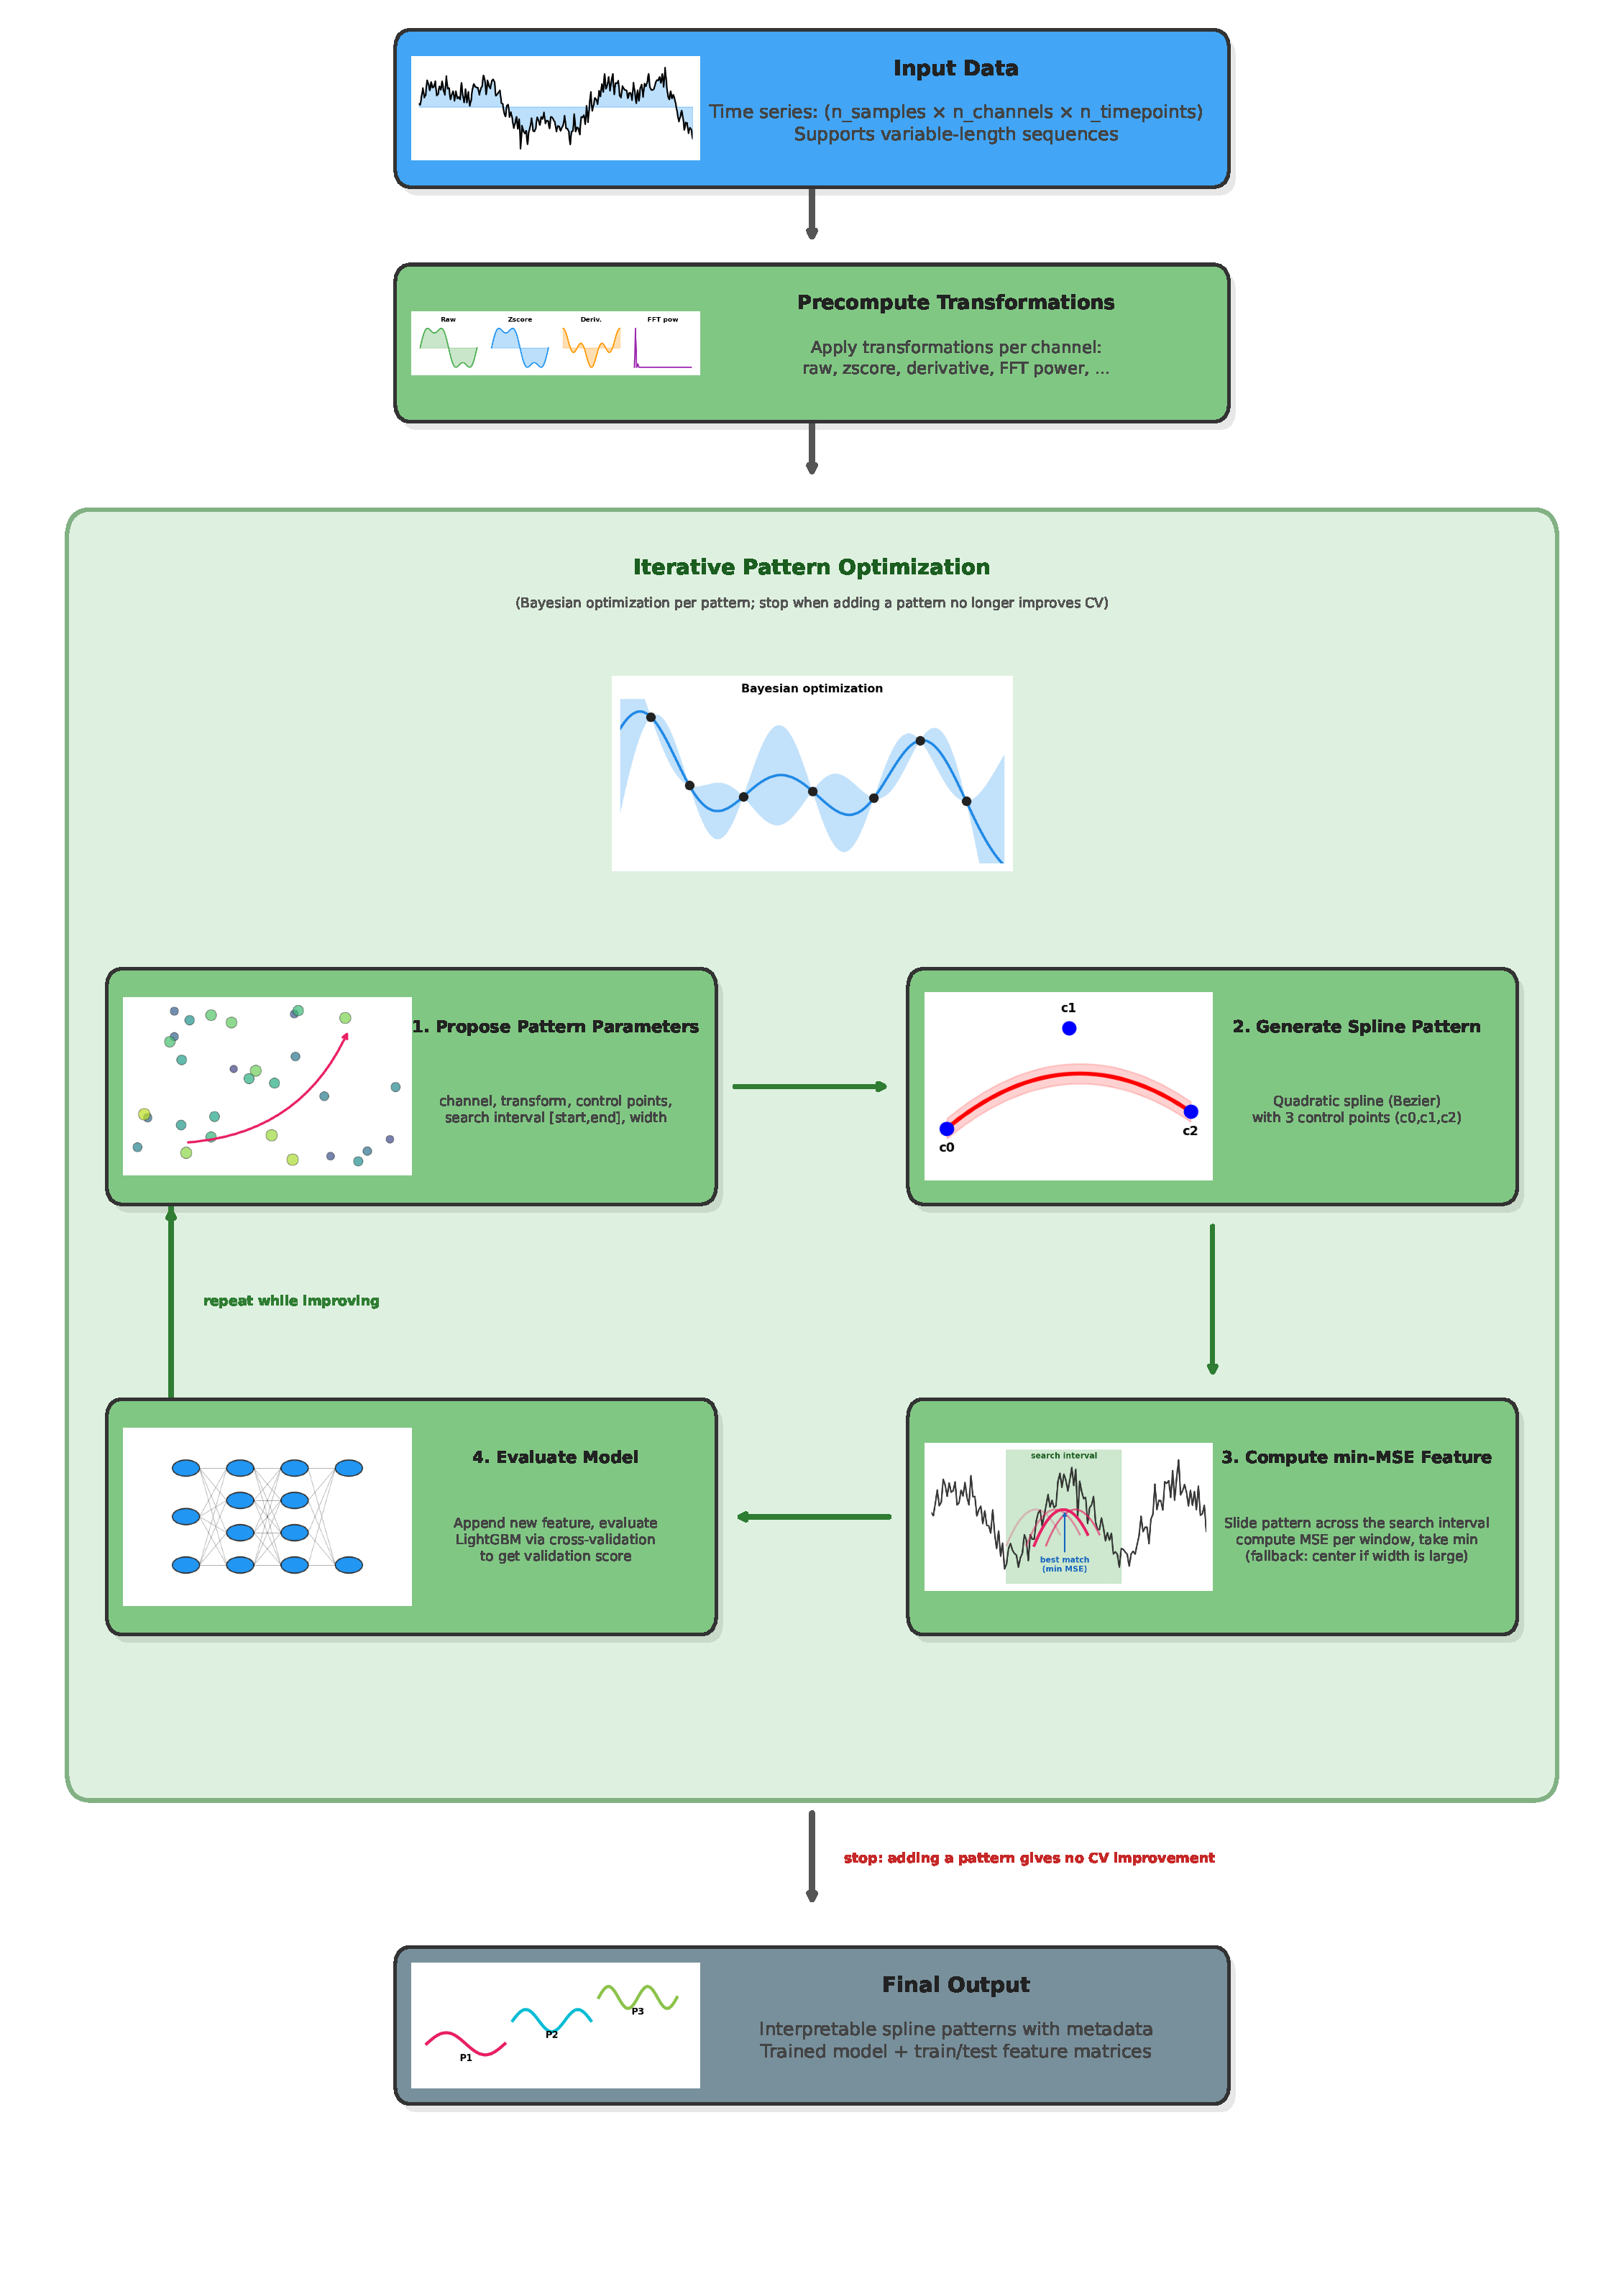
\includegraphics[width=0.65\textwidth,keepaspectratio]{images/flowchart/flowchart.pdf}
  \caption{patX methodology overview: The process begins with time series or
  spatial data, applies multiple signal transformations, and selects the top-K
  transforms via cross-validation.
  Pattern Characteristics Optimization then iteratively: (1) proposes N
  candidate patterns with parameters (channel, transform, control points,
  position, width), (2) generates smooth B-spline templates, (3) computes
  RMSE dissimilarity features between patterns and signal segments, and
  (4) evaluates model performance via cross-validation.
  Early stopping terminates when the validation score plateaus.
  Finally, backward elimination removes redundant patterns, yielding a compact
  set of interpretable patterns with a trained model for prediction.}
  \label{fig:patx_methodology}
\end{figure}

\subsection{Signal Transformation and Selection}
The first stage applies a set of signal transformations to all input channels,
creating multiple views of the data.
The default transformation library includes time-domain (raw, derivatives,
cumulative operations), frequency-domain (FFT, DCT), wavelet decompositions,
and nonlinear transforms---but users can define custom transformations for
domain-specific applications.

To focus the pattern search on the most informative representations, patX
evaluates each transformation independently.
For each transform, it computes aggregate statistics (mean, standard deviation,
skewness, kurtosis, quartiles, etc.) across all channels, then trains a model
using cross-validation.
The top-K transforms by validation score are retained for pattern optimization.
This automatic selection ensures patterns are discovered in the signal
representations most relevant to the prediction task.

\subsection{Pattern Characteristics Optimization}
The core of patX is an optimization loop that discovers discriminative patterns.
Each pattern is defined by five parameters:
\begin{enumerate}
\item \textbf{Channel index}: which input channel to examine (for multivariate
      data)
\item \textbf{Transform type}: which of the top-K transforms to use
\item \textbf{Control points}: values defining the B-spline shape
\item \textbf{Position}: where in the signal the pattern is located
\item \textbf{Width}: temporal extent of the pattern
\end{enumerate}

B-splines provide smooth, continuously differentiable curves controlled by a
small number of control points \cite{balestriero2018spline}.
Adjusting one control point affects only a local region of the curve, making
them ideal for representing localized temporal phenomena.
This is analogous to how convolutional neural networks learn local filters,
but with explicit, interpretable parameters.
The number of control points and spline degree are configurable.

The optimizer (e.g., Optuna's NSGA-II or TPE sampler) proposes N candidate
patterns per trial, each with randomly suggested parameters.
For each pattern, patX:
\begin{enumerate}
\item Generates a B-spline curve from the control points
\item Extracts the corresponding signal segment from the transformed data
\item Computes the RMSE between pattern and segment for all training samples
\end{enumerate}

To support spatially invariant pattern detection, patX can evaluate each
template in a sliding window over an allowed position range and use the best
match (minimum RMSE) as the feature value.
This is analogous to applying a convolutional filter across positions followed
by a global pooling operation: the learned template is reused at every offset,
and the pooling step makes the feature insensitive to small shifts.
When sliding is disabled, the template is evaluated at a single position,
producing position-specific features and removing width optimization.

These N RMSE values (one per pattern) become features for a machine learning
model, which is evaluated via inner cross-validation.
The validation score guides the optimizer toward better pattern configurations.
Optimization terminates when either the maximum number of trials is reached or
the validation score has not improved for a specified number of consecutive
trials (patience parameter).

\subsection{Backward Elimination}
After optimization, patX applies backward elimination to remove redundant
patterns.
Starting with all N optimized patterns, it iteratively:
\begin{enumerate}
\item Evaluates model performance when each pattern is removed
\item Removes the pattern whose absence least affects (or improves) performance
\item Repeats until removing any pattern would degrade performance beyond a
      tolerance threshold
\end{enumerate}

This yields a compact final set containing only patterns that provide measurable
predictive value.

\subsection{Output}
The final output consists of:
\begin{itemize}
\item A list of interpretable B-spline patterns with their parameters (channel,
      transform, control points, position, width)
\item A trained machine learning model
\item Feature matrices for train and test sets
\end{itemize}

Each pattern can be visualized by plotting its B-spline curve overlaid on
example signal segments, enabling domain experts to validate whether discovered
patterns correspond to known physiological or biological phenomena.

\subsection{Implementation Details}
Table~\ref{tab:implementation} summarizes the default configuration used in our
experiments.
All parameters are configurable; patX supports alternative optimizers,
machine learning models, B-spline configurations, and custom signal
transformations.
patX is available as an official Python package on PyPI
(\url{https://pypi.org/project/patx/}).

\begin{table}[H]
\centering
\caption{patX Default Configuration}
\label{tab:implementation}
\begin{tabular}{ll}
\toprule
\textbf{Component} & \textbf{Default Setting} \\
\midrule
Optimizer & Optuna with TPE sampler \\
Max Trials & 10,000 (early stopping patience: 1,000) \\
Patterns per Trial & 15 \\
B-spline Degree & Cubic (degree 3) \\
Control Points & 3 per pattern \\
Transforms Library & 20 built-in (raw, derivative, FFT, wavelets, etc.) \\
Transforms Selected & Top-5 by CV performance \\
Inner CV Folds & 3 \\
Max Samples (search) & 2,000 \\
ML Model & XGBoost \\
\bottomrule
\end{tabular}
\end{table}

The built-in transformation library includes: raw, derivative, second
derivative, cumulative sum, difference, log1p, absolute value, sorted, DCT,
FFT power, exponential, tanh, sin, cos, reciprocal, autocorrelation, and
wavelet decompositions (db4, sym4, coif1, haar).
Users can extend this library with domain-specific transformations.
We ran our experiments on a MacBook Pro M2 using 12 cores and 32GB of RAM. 

\subsection{Datasets}
We evaluate patX across seven diverse biomedical datasets spanning glucose
forecasting, arrhythmia classification, emotion classification, gene expression
prediction, clinical outcome prediction, human activity recognition, and voice
pathology detection.
Table~\ref{tab:datasets} summarizes the key characteristics of each dataset.

\begin{table}[H]
\centering
\caption{Dataset Characteristics and Evaluation Metrics}
\label{tab:datasets}
\footnotesize
\begin{tabular*}{\textwidth}{@{\extracolsep{\fill}}lccccll@{}}
\toprule
\textbf{Dataset} & \textbf{Samples} & \textbf{Chan.} & \textbf{Length} &
\textbf{Metric} & \textbf{Input Data} & \textbf{Target Feature} \\
\midrule
AZT1D & $\sim$12k & 3 & 24 & RMSE & CGM, Insulin, Carbs & Future glucose
change \\
MITBIH & $\sim$12k & 1 & 100 & Acc. & ECG beats & 5--class arrhythmia type \\
Emotions & 2,048 & 5 & 254 & AUC & EEG channels & 3--class emotion state \\
REMC & 18,421 & 5 & 200 & AUC & Histone marks & Gene expression
(high/low) \\
MIMIC--IV & $\sim$4k & 29 & 24 & AUC & EHR time series & ARDS diagnosis \\
PAMAP2 & $\sim$4k & 51 & 100 & Acc. & IMU sensors & 12--class activity type \\
SVD & $\sim$2k & 3 & 700 & AUC & Sustained vowels (/a/,/i/,/u/) &
Healthy vs.\ pathology \\
\bottomrule
\end{tabular*}
\end{table}

\textbf{AZT1D (glucose forecasting).}
Glucose change prediction from 24 lagged timepoints (2h history) of CGM, insulin,
and carbohydrate signals, with physiological response curve modeling for delayed
effects (see Supplementary Figure~\ref{fig:azt1d_preprocessing}).
Link: \url{https://data.mendeley.com/datasets/gk9m674wcx/1}.

\textbf{MITBIH (arrhythmia classification).}
We extract 100-sample ECG beats centered on R-peaks, classifying into five
arrhythmia types (N, L, R, A, V) with random undersampling for class balance.
Link: \url{https://www.kaggle.com/datasets/mondejar/mitbih-database}.

\textbf{Emotions (EEG emotion classification).}
EEG recordings (254 time points, 5 channels) during emotional states,
classified into positive, neutral, and negative emotions.
Link: \href{https://kaggle.com/datasets/birdy654/eeg-brainwave-dataset-feeling-emotions}
{Kaggle dataset}.

\textbf{REMC (ChIP-seq gene expression).}
Binary gene expression prediction from five histone marks (H3K4me1, H3K4me3,
H3K36me3, H3K9me3, H3K27me3) across 200 bins around the TSS for 18,421 genes.
Data: \url{https://egg2.wustl.edu/roadmap/web_portal/processed_data.html}.

\textbf{MIMIC--IV (ARDS classification).}
ARDS prediction from 29 clinical time series (vitals, labs, ventilator settings)
over 24 hourly bins per ICU patient \cite{Johnson2023MIMICIV}.
Link: \url{https://physionet.org/content/mimiciv/3.1/}.

\textbf{PAMAP2 (activity recognition).}
Activity classification from 51 IMU channels (3 sensors $\times$ 17 features)
using 100-sample windows across 12 activity classes from 9 subjects
\cite{Reiss2012PAMAP2}.

\textbf{SVD (voice pathology detection).}
Binary classification of healthy versus pathological voice recordings from the
Saarbr\"ucken Voice Database (SVD), following the methodology of Lee
\cite{lee2021experimental}.
We select 259 healthy and 259 pathological recordings per gender at normal
pitch for sustained vowels /a/, /i/, and /u/.
Female pathologies include hyperfunctional dysphonia (97), functional dysphonia
(51), laryngitis (30), and others (81); male pathologies include laryngitis
(62), hyperfunctional dysphonia (44), vocal fold polyp (25), and others (128).
Raw audio waveforms are bandpass filtered (80--4000~Hz), pre-emphasized,
silence-trimmed, and resampled to 700 samples per vowel.
Following established protocols, we perform separate evaluations by gender
and vowel to account for physiological differences in vocal characteristics
\cite{martinez2012voice, huckvale2021automated}.
Link: \url{https://zenodo.org/records/16874898}.

\subsection{Baselines}
We compare patX against three established approaches for time series analysis:
tsfresh and catch22 for automated feature extraction combined with XGBoost,
and a 1D convolutional neural network for end--to--end learning.

\subsubsection{TSFRESH and catch22 Baselines}
For tsfresh, we use \texttt{MinimalFCParameters} to extract compact descriptors
including moments, spectral features, and shape statistics, training XGBoost
on all extracted features.
For catch22, we extract the 22 canonical features from the library
\cite{lubba2019catch22} and train XGBoost \cite{chen2016xgboost}.
Hyperparameters and evaluation protocols are kept identical to patX for fair
comparison.

\subsubsection{CNN Baseline Implementation}
We implement a 1D CNN using PyTorch with three convolutional layers
(filters: 64, 128, 256) each containing convolution, batch normalization, ReLU,
max pooling, and dropout.
The architecture uses kernel sizes of 7, 5, and 3 for the three layers
respectively, with appropriate padding to maintain temporal resolution.
Adaptive average pooling aggregates features across the temporal dimension,
followed by fully connected layers (256→128→64→output) with ReLU activations,
batch normalization, and dropout (0.4, 0.3) for regularization.
We train with Adam optimizer (lr=0.1, weight decay=1e-4), early stopping
(patience=10), and learning rate reduction on plateau (factor=0.5, patience=3).
For binary classification tasks, we use cross-entropy loss with class weights
computed to handle imbalanced datasets; for multi-class classification and
regression, we use unweighted cross-entropy and MSE loss respectively.
The model automatically detects the number of input channels based on the
dataset structure: 3 channels for AZT1D (CGM, insulin, carbs), 5 channels for
REMC (histone marks), and 1 channel for univariate time series.
Training uses 100 epochs maximum with batch size 128, matching evaluation
protocols with other baselines.

\subsection{Evaluation}
For datasets using cross-validation, we use 5--fold stratified splits with
fixed seeds.
For subject-level datasets (AZT1D, PAMAP2), we use 70\%/30\% train/test splits
per subject.
Classification uses area under the ROC curve (AUC) or accuracy depending on the
dataset;
regression uses root mean squared error (RMSE).
We report the number of extracted patterns alongside predictive performance as
mean $\pm$ standard deviation across folds or subjects.

\section{Results}

\subsection{Performance Comparison}

\begin{table}[H]
\centering
\caption{Performance comparison across biomedical datasets. Results show mean $\pm$ standard deviation across subjects/folds. Best performance per dataset highlighted in bold.}
\label{tab:results}
\footnotesize
\begin{tabular*}{\textwidth}{@{\extracolsep{\fill}}lccccc@{}}
\toprule
\textbf{Dataset} & \textbf{Method} & \textbf{Score} & \textbf{Features} & \textbf{Time (s)} \\
\midrule
AZT1D & PATX & \textbf{22.460 $\pm$ 5.965} & 9.9 $\pm$ 6.0 & 448.3 $\pm$ 713.3 \\
 & TSFRESH & 32.546 $\pm$ 4.961 & 11.0 & 1.8 $\pm$ 0.2 \\
 & CATCH22 & 32.342 $\pm$ 4.808 & 23.0 & 2.9 $\pm$ 0.4 \\
 & CNN & 29.898 $\pm$ 4.500 & 73.0 & 26.7 $\pm$ 14.4 \\
\addlinespace
Emotions & PATX & \textbf{0.917 $\pm$ 0.013} & 5.6 $\pm$ 1.7 & 203.7 $\pm$ 53.9 \\
 & TSFRESH & 0.904 $\pm$ 0.008 & 10.0 & 1.1 $\pm$ 0.1 \\
 & CATCH22 & 0.876 $\pm$ 0.005 & 22.0 & 14.8 $\pm$ 0.9 \\
 & CNN & 0.668 $\pm$ 0.001 & 1500.0 & 3.4 $\pm$ 1.2 \\
\addlinespace
MIMIC-IV & PATX & \textbf{0.781 $\pm$ 0.013} & 6.0 $\pm$ 2.1 & 151.7 $\pm$ 42.7 \\
 & TSFRESH & 0.738 $\pm$ 0.007 & 10.0 & 1.2 $\pm$ 0.0 \\
 & CATCH22 & 0.752 $\pm$ 0.003 & 22.0 & 9.0 $\pm$ 0.2 \\
 & CNN & 0.774 $\pm$ 0.003 & 696.0 & 3.5 $\pm$ 0.6 \\
\addlinespace
MITBIH & PATX & \textbf{0.948 $\pm$ 0.004} & 11.8 $\pm$ 3.0 & 933.7 $\pm$ 278.4 \\
 & TSFRESH & 0.527 $\pm$ 0.008 & 10.0 & 2.1 $\pm$ 0.0 \\
 & CATCH22 & 0.710 $\pm$ 0.013 & 22.0 & 4.0 $\pm$ 0.0 \\
 & CNN & 0.942 $\pm$ 0.004 & 100.0 & 36.8 $\pm$ 9.5 \\
\addlinespace
REMC & PATX & 0.936 $\pm$ 0.012 & 10.7 $\pm$ 2.7 & 220.5 $\pm$ 54.3 \\
 & TSFRESH & 0.878 $\pm$ 0.015 & 10.0 & 6.1 $\pm$ 0.1 \\
 & CATCH22 & 0.906 $\pm$ 0.015 & 22.0 & 54.1 $\pm$ 2.0 \\
 & CNN & \textbf{0.943 $\pm$ 0.011} & 1000.0 & 18.0 $\pm$ 4.5 \\
\addlinespace
PAMAP2 & PATX & \textbf{0.997 $\pm$ 0.001} & 8.4 $\pm$ 1.8 & 8452.1 $\pm$ 5237.6 \\
 & TSFRESH & 0.465 $\pm$ 0.005 & 10.0 & 9.8 $\pm$ 0.3 \\
 & CATCH22 & 0.484 $\pm$ 0.005 & 22.0 & 93.5 $\pm$ 4.8 \\
 & CNN & 0.987 $\pm$ 0.002 & 520.0 & 267.3 $\pm$ 40.8 \\
\addlinespace
SVD & PATX & \textbf{0.588 $\pm$ 0.019} & 3.0 $\pm$ 1.2 & 76.8 $\pm$ 10.2 \\
 & TSFRESH & 0.576 $\pm$ 0.011 & 10.0 & 2.4 $\pm$ 0.1 \\
 & CATCH22 & 0.570 $\pm$ 0.015 & 22.0 & 55.6 $\pm$ 2.1 \\
 & CNN & 0.570 $\pm$ 0.004 & 6300.0 & 1.3 $\pm$ 1.1 \\
\bottomrule
\end{tabular*}
\end{table}


Table~\ref{tab:results} presents the test set performance of patX + XGBoost,
tsfresh + XGBoost, catch22 + XGBoost, and CNN baselines across seven
biomedical datasets, now including the Saarbr\"ucken Voice Database (SVD) for
healthy vs.\ diseased voice pathology detection.

patX achieves the best overall performance on six of seven datasets
(AZT1D, Emotions, MIMIC-IV, MITBIH, PAMAP2, and SVD).
On REMC, the CNN baseline slightly outperforms patX (0.935 vs.\ 0.928).
The gains are especially pronounced on AZT1D glucose forecasting, where patX
reduces RMSE from 29.9 (CNN) and 32.5 (tsfresh) to 22.5 while using about
10 patterns on average.

We focus on two aspects: predictive performance and feature transparency.
patX produces a compact set of explicit templates and turns their matches into
features, enabling direct visualization and domain validation.
As a result, the model's decision inputs can be inspected in the same units as
the original signals (or their selected transforms).

\subsection{Ablation Study}
We ablate key components across MITBIH (accuracy), SVD (AUC), and REMC (AUC)
using the same gradient boosting classifier and 5-fold stratified splits used throughout.
Table~\ref{tab:ablation} reports mean $\pm$ std for score, runtime, and feature
count.

\begin{table}[H]
\centering
\caption{Ablation study across MITBIH (accuracy), SVD (AUC), and REMC (AUC).
Mean $\pm$ std over folds (5 for MITBIH; 2 for SVD and REMC).}
\label{tab:ablation}
\footnotesize
\tiny
\renewcommand{\arraystretch}{0.75}
\begin{tabular*}{\textwidth}{@{\extracolsep{0.5pt}}l|c|c|c|c|c|c|c@{}}
\toprule
\textbf{Dataset} & \textbf{Baseline} & \textbf{Trials=100} & \textbf{No Transforms} & \textbf{CP=1} & \textbf{Linear Model} & \textbf{No Sliding} & \textbf{Polynomial} \\
\midrule
MITBIH & \makecell{0.947 $\pm$ 0.004 \\\\ Feat: 14.8 $\pm$ 2.2} & \makecell{0.944 $\pm$ 0.004 \\\\ Feat: 16.4 $\pm$ 3.0} & \makecell{0.907 $\pm$ 0.006 \\\\ Feat: 12.4 $\pm$ 3.0} & \makecell{0.948 $\pm$ 0.004 \\\\ Feat: 16.4 $\pm$ 1.8} & \makecell{0.828 $\pm$ 0.045 \\\\ Feat: 16.0 $\pm$ 3.5} & \makecell{0.946 $\pm$ 0.002 \\\\ Feat: 15.6 $\pm$ 3.2} & \makecell{\textbf{0.951 $\pm$ 0.003} \\\\ Feat: 18.0 $\pm$ 2.4} \\
\midrule
SVD & \makecell{0.597 $\pm$ 0.026 \\\\ Feat: 3.0 $\pm$ 1.2} & \makecell{0.578 $\pm$ 0.033 \\\\ Feat: 3.4 $\pm$ 1.9} & \makecell{0.574 $\pm$ 0.030 \\\\ Feat: 4.0 $\pm$ 1.0} & \makecell{0.574 $\pm$ 0.021 \\\\ Feat: 4.0 $\pm$ 0.7} & \makecell{0.581 $\pm$ 0.041 \\\\ Feat: 3.0 $\pm$ 0.7} & \makecell{\textbf{0.603 $\pm$ 0.023} \\\\ Feat: 3.2 $\pm$ 1.6} & \makecell{0.589 $\pm$ 0.029 \\\\ Feat: 3.8 $\pm$ 1.3} \\
\midrule
Emotions & \makecell{0.986 $\pm$ 0.005 \\\\ Feat: 7.4 $\pm$ 1.3} & \makecell{0.980 $\pm$ 0.004 \\\\ Feat: 7.6 $\pm$ 2.7} & \makecell{0.921 $\pm$ 0.017 \\\\ Feat: 6.8 $\pm$ 1.9} & \makecell{0.983 $\pm$ 0.005 \\\\ Feat: 8.8 $\pm$ 0.8} & \makecell{0.752 $\pm$ 0.035 \\\\ Feat: 7.8 $\pm$ 1.3} & \makecell{0.985 $\pm$ 0.005 \\\\ Feat: 8.8 $\pm$ 2.2} & \makecell{\textbf{0.987 $\pm$ 0.004} \\\\ Feat: 10.0 $\pm$ 2.3} \\
\midrule
MIMIC-IV & \makecell{\textbf{0.767 $\pm$ 0.010} \\\\ Feat: 6.2 $\pm$ 2.6} & \makecell{0.767 $\pm$ 0.013 \\\\ Feat: 6.6 $\pm$ 2.2} & \makecell{0.763 $\pm$ 0.008 \\\\ Feat: 3.2 $\pm$ 1.1} & \makecell{0.762 $\pm$ 0.016 \\\\ Feat: 5.8 $\pm$ 0.4} & \makecell{0.743 $\pm$ 0.001 \\\\ Feat: 4.2 $\pm$ 1.9} & \makecell{0.756 $\pm$ 0.013 \\\\ Feat: 2.8 $\pm$ 2.5} & \makecell{0.759 $\pm$ 0.014 \\\\ Feat: 3.6 $\pm$ 2.5} \\
\midrule
PAMAP2 & \makecell{0.996 $\pm$ 0.001 \\\\ Feat: 9.0 $\pm$ 1.0} & \makecell{0.991 $\pm$ 0.001 \\\\ Feat: 7.4 $\pm$ 1.7} & \makecell{0.997 $\pm$ 0.000 \\\\ Feat: 7.2 $\pm$ 0.8} & \makecell{0.997 $\pm$ 0.001 \\\\ Feat: 7.4 $\pm$ 0.5} & \makecell{0.996 $\pm$ 0.001 \\\\ Feat: 7.0 $\pm$ 1.0} & \makecell{0.996 $\pm$ 0.001 \\\\ Feat: 7.4 $\pm$ 0.9} & \makecell{\textbf{0.997 $\pm$ 0.001} \\\\ Feat: 7.4 $\pm$ 1.5} \\
\midrule
REMC & \makecell{0.928 $\pm$ 0.003 \\\\ Feat: 13.2 $\pm$ 2.2} & \makecell{0.927 $\pm$ 0.005 \\\\ Feat: 14.6 $\pm$ 5.8} & \makecell{\textbf{0.930 $\pm$ 0.003} \\\\ Feat: 15.8 $\pm$ 3.8} & \makecell{0.929 $\pm$ 0.005 \\\\ Feat: 13.2 $\pm$ 4.6} & --- & --- & --- \\
\bottomrule
\end{tabular*}

\end{table}

The ablations isolate which components contribute most to performance.
On MITBIH, disabling shifting causes the largest drop (0.888 vs.\ 0.940),
indicating that translation-invariant matching is important for aligning beat
morphology.
Increasing the optimization budget yields modest gains: 1000 trials improves
accuracy to 0.944 but increases runtime substantially, while 100 trials remains
competitive (0.941) with much lower cost.
Reducing expressiveness to a single control point also degrades performance
(0.928), suggesting that non-trivial templates are needed.

On REMC (E003), performance is relatively stable across variants.
No shifting does not hurt (0.923), consistent with patterns being anchored near
the TSS.
The best configuration uses a smaller optimization budget (100 trials, 0.925),
suggesting diminishing returns from additional search on this task.

On SVD, the optimization strategy has a strong effect: parallel optimization
achieves the best AUC (0.594) and reduces runtime relative to the baseline.
No shifting performs similarly to baseline (0.563 vs.\ 0.549), while a single
control point is insufficient (0.505).

\subsection{Domain-Specific Pattern Interpretation}

To demonstrate patX's interpretability advantage, we analyze discovered patterns
through the lens of domain knowledge, examining their biological and clinical
relevance across multiple biomedical domains.
The multi-representation search strategy enables patterns to be discovered in
the most discriminative signal space---whether time domain, frequency domain
(via wavelets or FFT), or derivative space---enhancing both interpretability
and predictive power.

Figure~\ref{fig:domain_pattern_interpretation} presents a comprehensive
visualization of pattern discovery in the REMC dataset, focusing on the H3K4me3
histone mark in cell line E003.
The analysis is decomposed into four panels to illustrate the complete feature
extraction process:
(a) Raw input signals for representative high and low expression genes, showing
H3K4me3 enrichment around the transcription start site (TSS).
(b) The transformed signal space (cumulative sum) where pattern matching occurs,
with the learned B-spline template overlaid at its optimal position.
The cumsum transformation captures the total accumulation of histone marks,
which is significantly higher for active promoters.
(c) Average class profiles (mean $\pm$ std) demonstrating the global difference
in cumulative H3K4me3 signal between high and low expression genes, with the
pattern targeting the region of maximal divergence.
(d) The distribution of RMSE values, showing clear separation between classes
based on their similarity to the learned template.
This multi-view visualization confirms that patX discovers biologically
meaningful patterns (H3K4me3 accumulation) and uses them to construct
discriminative features in an interpretable manner.

\begin{figure}[H]
  \centering
  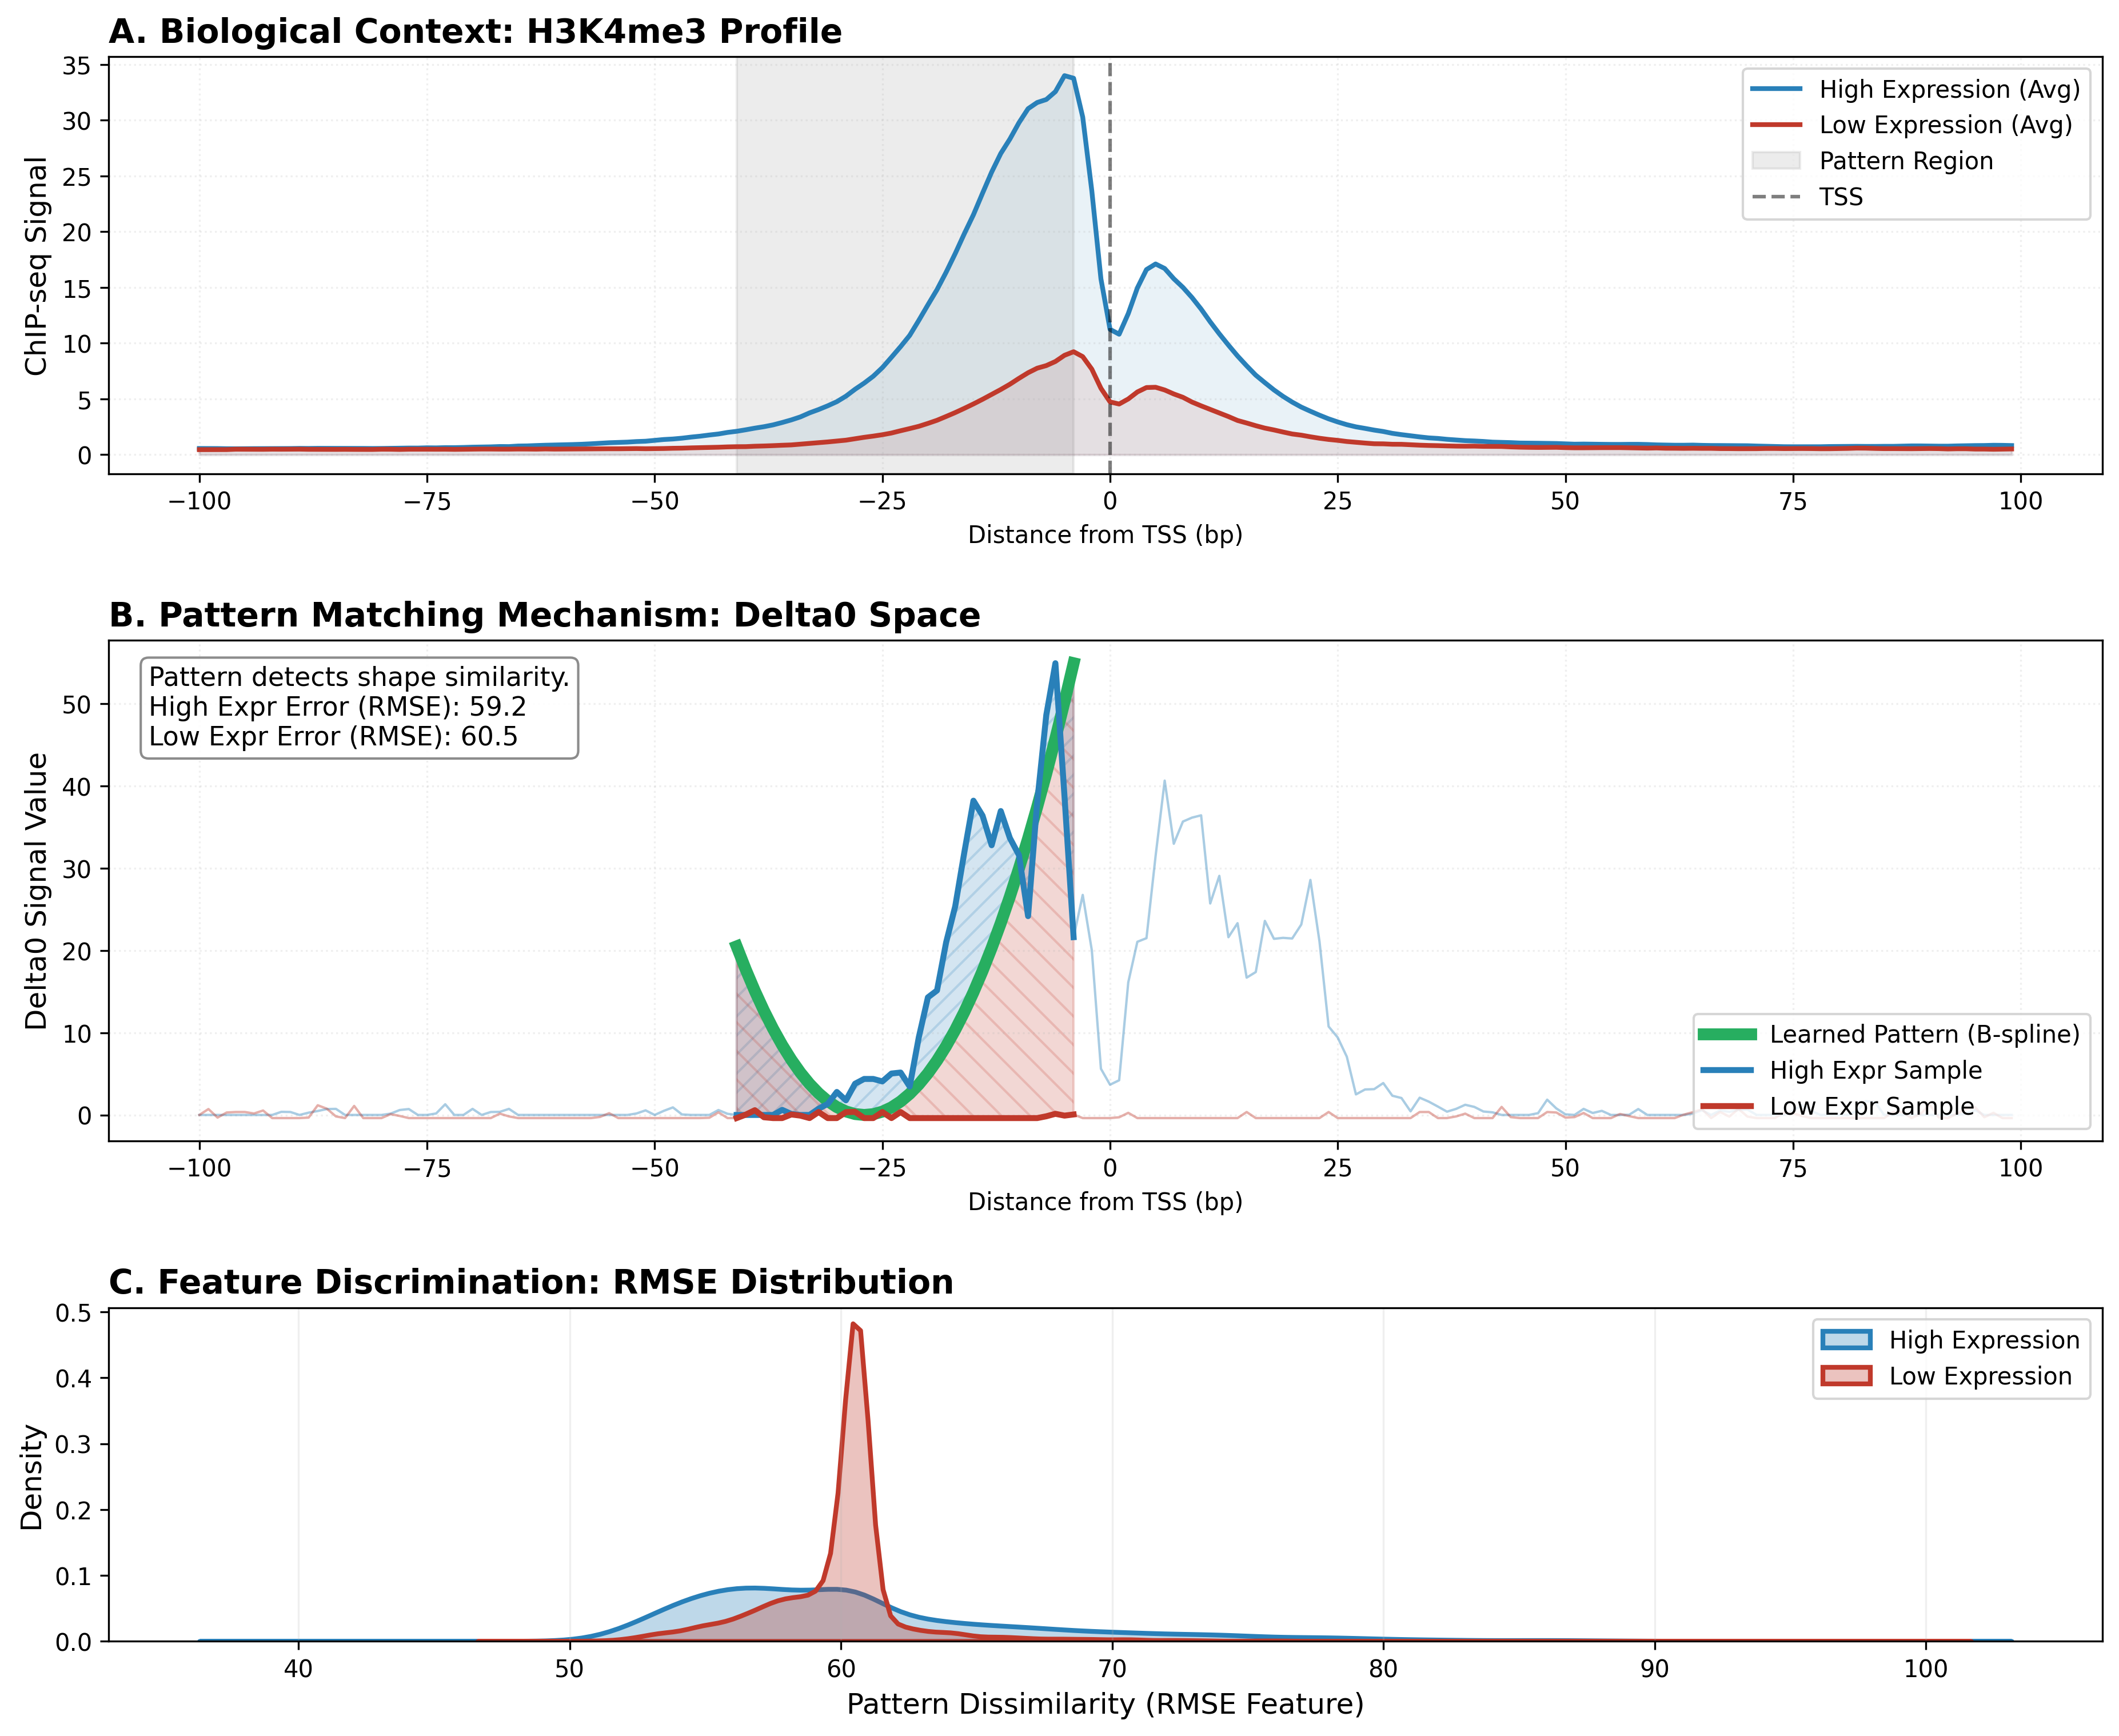
\includegraphics[width=\textwidth,keepaspectratio]
  {images/domain_pattern_interpretation.png}
  \caption{Domain-specific pattern interpretation for REMC (H3K4me3).
  The four panels illustrate the pattern extraction mechanism:
  (Top-Left) Raw ChIP-seq signals for representative high (blue) and low (red)
  expression genes around the TSS.
  (Top-Right) Transformed signals (cumulative sum) with the learned B-spline
  pattern (green) overlaid at its optimal matching position.
  (Bottom-Left) Average profiles for high and low expression classes with
  standard deviation shading, showing how the pattern aligns with the global
  difference in H3K4me3 accumulation.
  (Bottom-Right) Distribution of RMSE features, demonstrating discriminative
  separation between gene expression classes based on pattern similarity.}
  \label{fig:domain_pattern_interpretation}
\end{figure}

\subsubsection{Individual Prediction Explainability via SHAP Analysis}

To demonstrate patX's explainability at the individual prediction level, we
perform SHAP (SHapley Additive exPlanations) analysis
\cite{lundberg2017unified, mosca2022shap}
on a representative high-expression gene from REMC (E003).
Figure~\ref{fig:shap_waterfall_combined} shows how discovered histone patterns
combine to predict gene expression.

The resulting attributions can often be related to known biology.
For example, patterns linked to promoter-associated marks (e.g., H3K4me3) tend
to support predictions of active genes, while patterns linked to repressive
marks (e.g., H3K27me3) tend to support the opposite direction
\cite{heintzman2007distinct, barski2007high}.
The automatic selection of both raw (profile shape) and cumulative
transformations illustrates how patX can capture complementary signal aspects
without manual specification.

\begin{figure}[H]
  \centering
  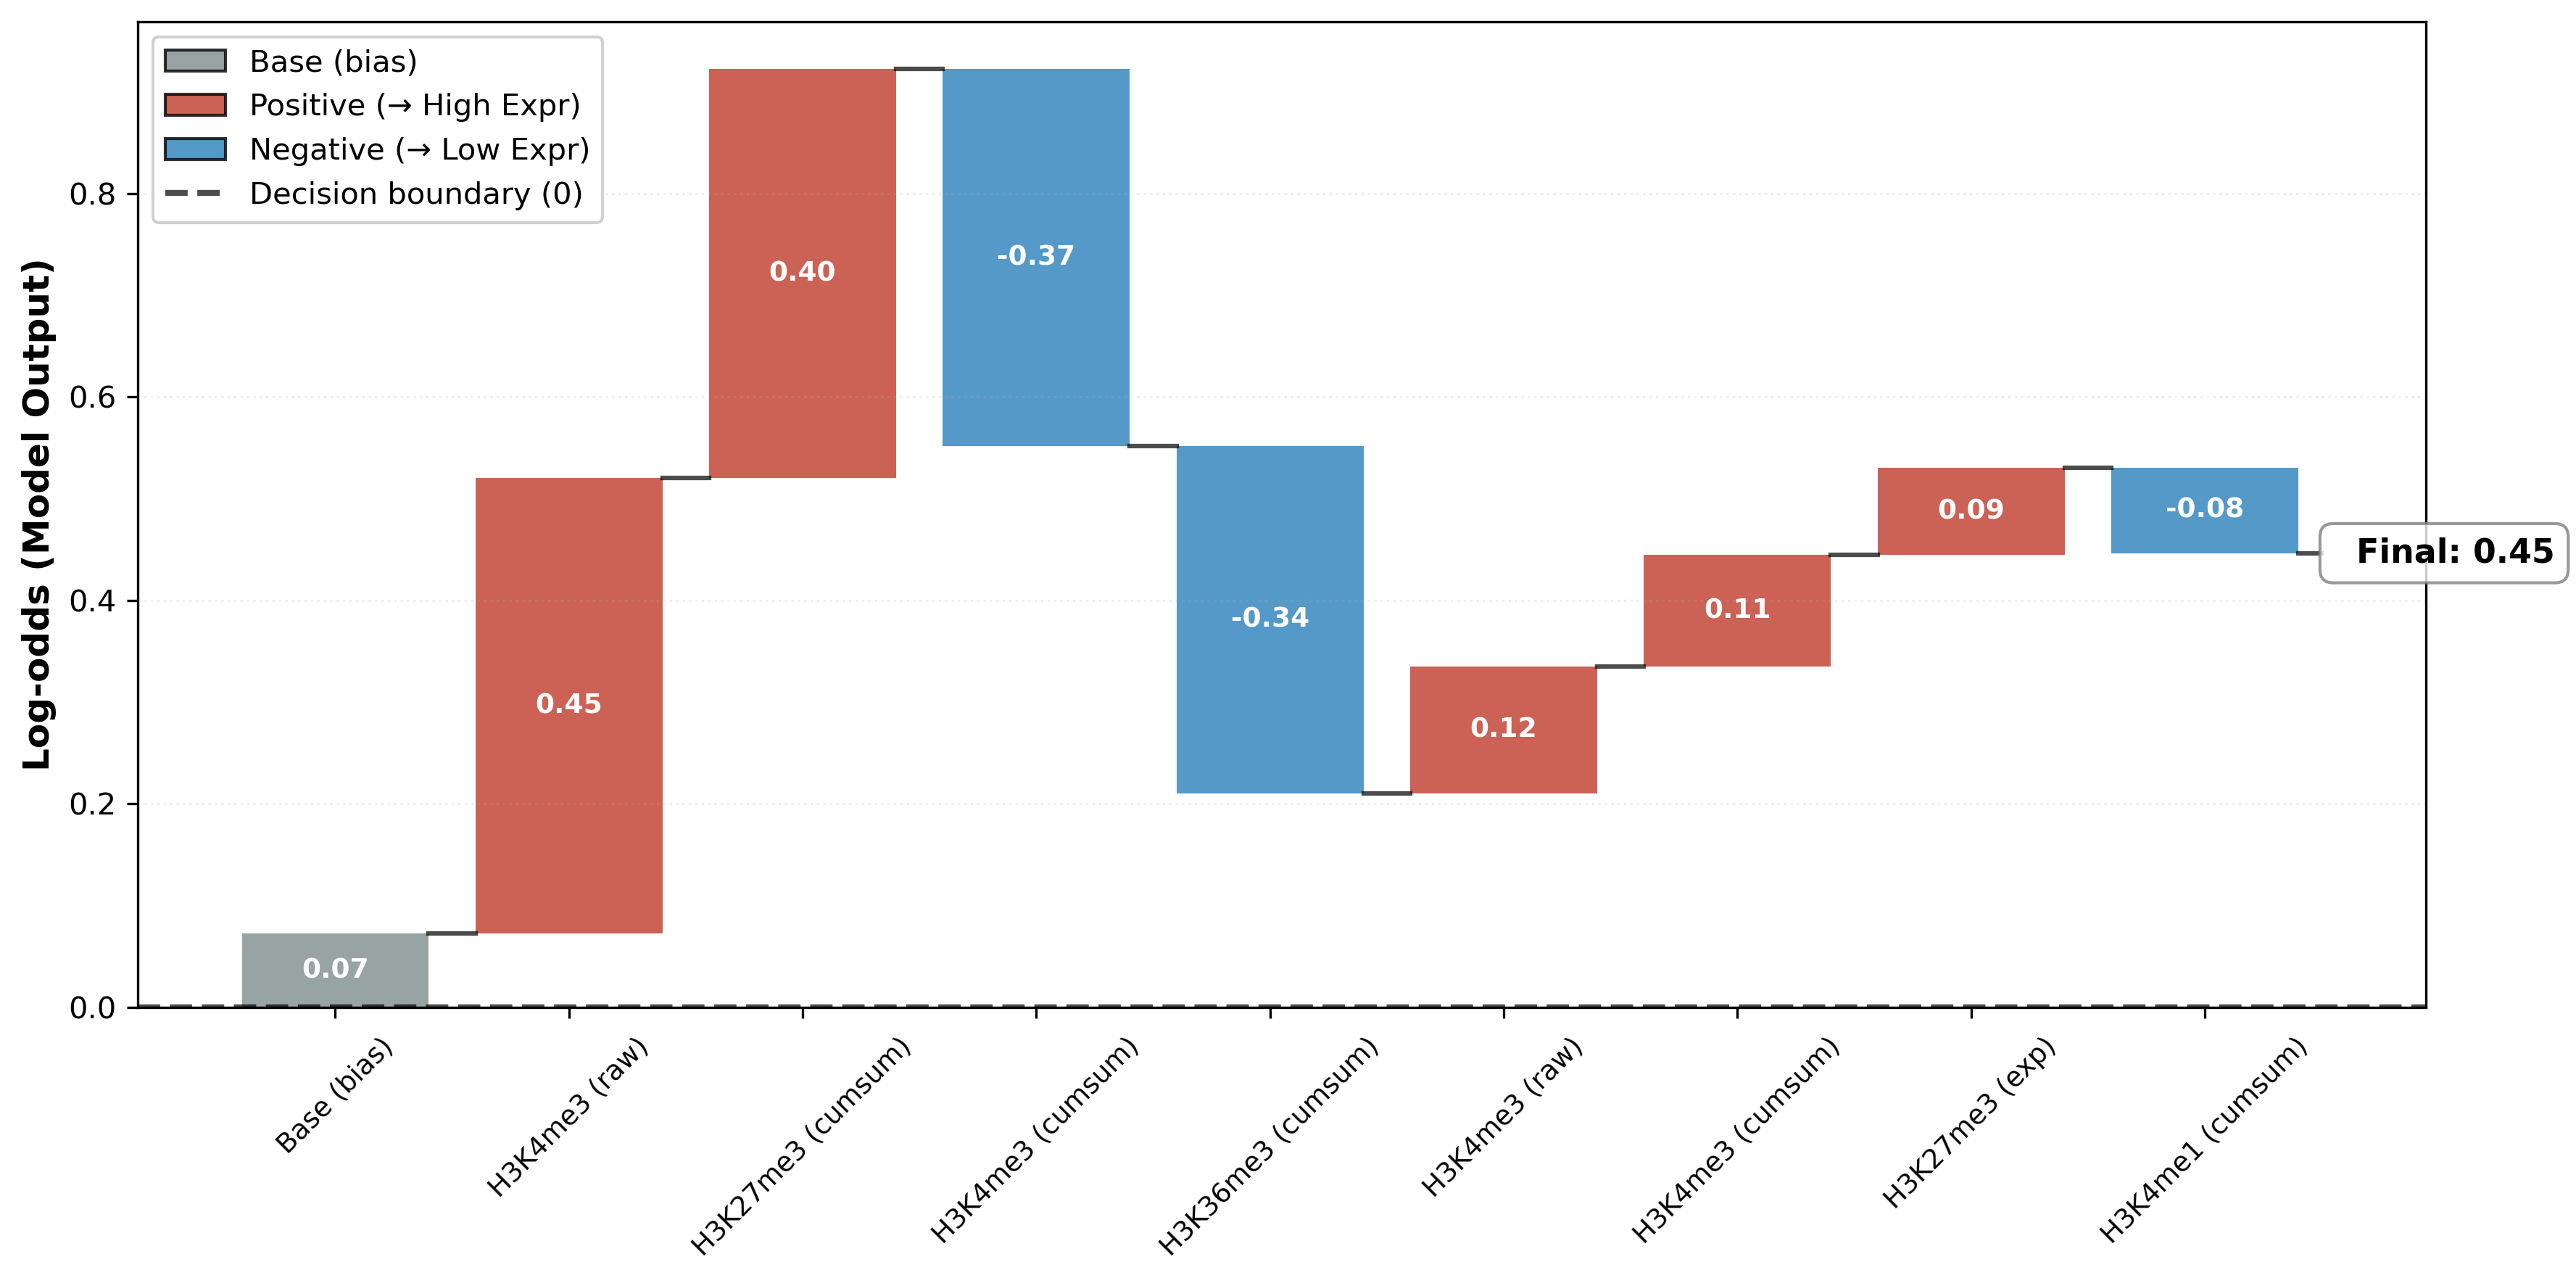
\includegraphics[width=\textwidth,keepaspectratio]
  {images/shap_waterfall.png}
  \caption{SHAP waterfall plot for gene expression prediction in REMC (E003).
  Each bar shows a pattern's contribution to the final log-odds prediction.
  Feature labels indicate the histone mark and transformation type.
  Positive contributions (red) push towards high expression; negative (blue)
  towards low expression.}
  \label{fig:shap_waterfall_combined}
\end{figure}

\subsection{Pattern Stability and Reproducibility}

To evaluate patX's robustness, we analyze pattern consistency across
cross-validation folds and subjects.
Table~\ref{tab:pattern_stability} reports the number of selected patterns
(mean $\pm$ std) and the dominant transformation and channel of the most
important pattern with consistency percentages.
Single-channel datasets (MITBIH, Emotions) show ``---'' for channel consistency.

Across datasets, we observe that some tasks favor a small set of dominant
transformations or channels, while others show more diversity.
This aligns with differences in signal structure: some problems have a clear
dominant representation (e.g., rate-of-change or frequency content), whereas
others distribute discriminative information across channels and transforms.

Figure~\ref{fig:pattern_stability} visualizes the primary pattern from each
fold for REMC (E003), showing consistent positioning near the transcription
start site despite variation in histone mark selection.

\begin{table}[H]
\centering
\caption{Pattern discovery characteristics across datasets. For each dataset, we report
the number of selected patterns (mean $\pm$ std across folds/subjects), and the dominant
transformation and channel of the most important pattern with consistency percentages.
Single-channel datasets show ``---'' for channel consistency.}
\label{tab:pattern_stability}
\footnotesize
\begin{tabular*}{\textwidth}{@{\extracolsep{\fill}}lccc@{}}
\toprule
\textbf{Dataset} & \textbf{Patterns} & \textbf{Transform (consistency)} & \textbf{Channel (consistency)} \\
\midrule
MITBIH & 11.8 $\pm$ 2.7 & pct\_change (60\%) & ECG (---) \\
EMOTIONS & 5.6 $\pm$ 1.5 & preemph97 (60\%) & EEG (60\%) \\
MIMIC & 6.0 $\pm$ 1.9 & dct (100\%) & pao2 (40\%) \\
PAMAP2 & 8.4 $\pm$ 1.6 & sorted (40\%) & heart\_rate (20\%) \\
SVD & 2.4 $\pm$ 1.5 & ecg\_resp (20\%) & a\_n\_mfcc1 (60\%) \\
REMC (E003) & 11.6 $\pm$ 1.4 & delta0 (40\%) & H3K4me3 (100\%) \\
AZT1D & 6.4 $\pm$ 1.3 & raw (29\%) & CGM (62\%) \\
\bottomrule
\end{tabular*}
\end{table}

\begin{figure}[H]
  \centering
  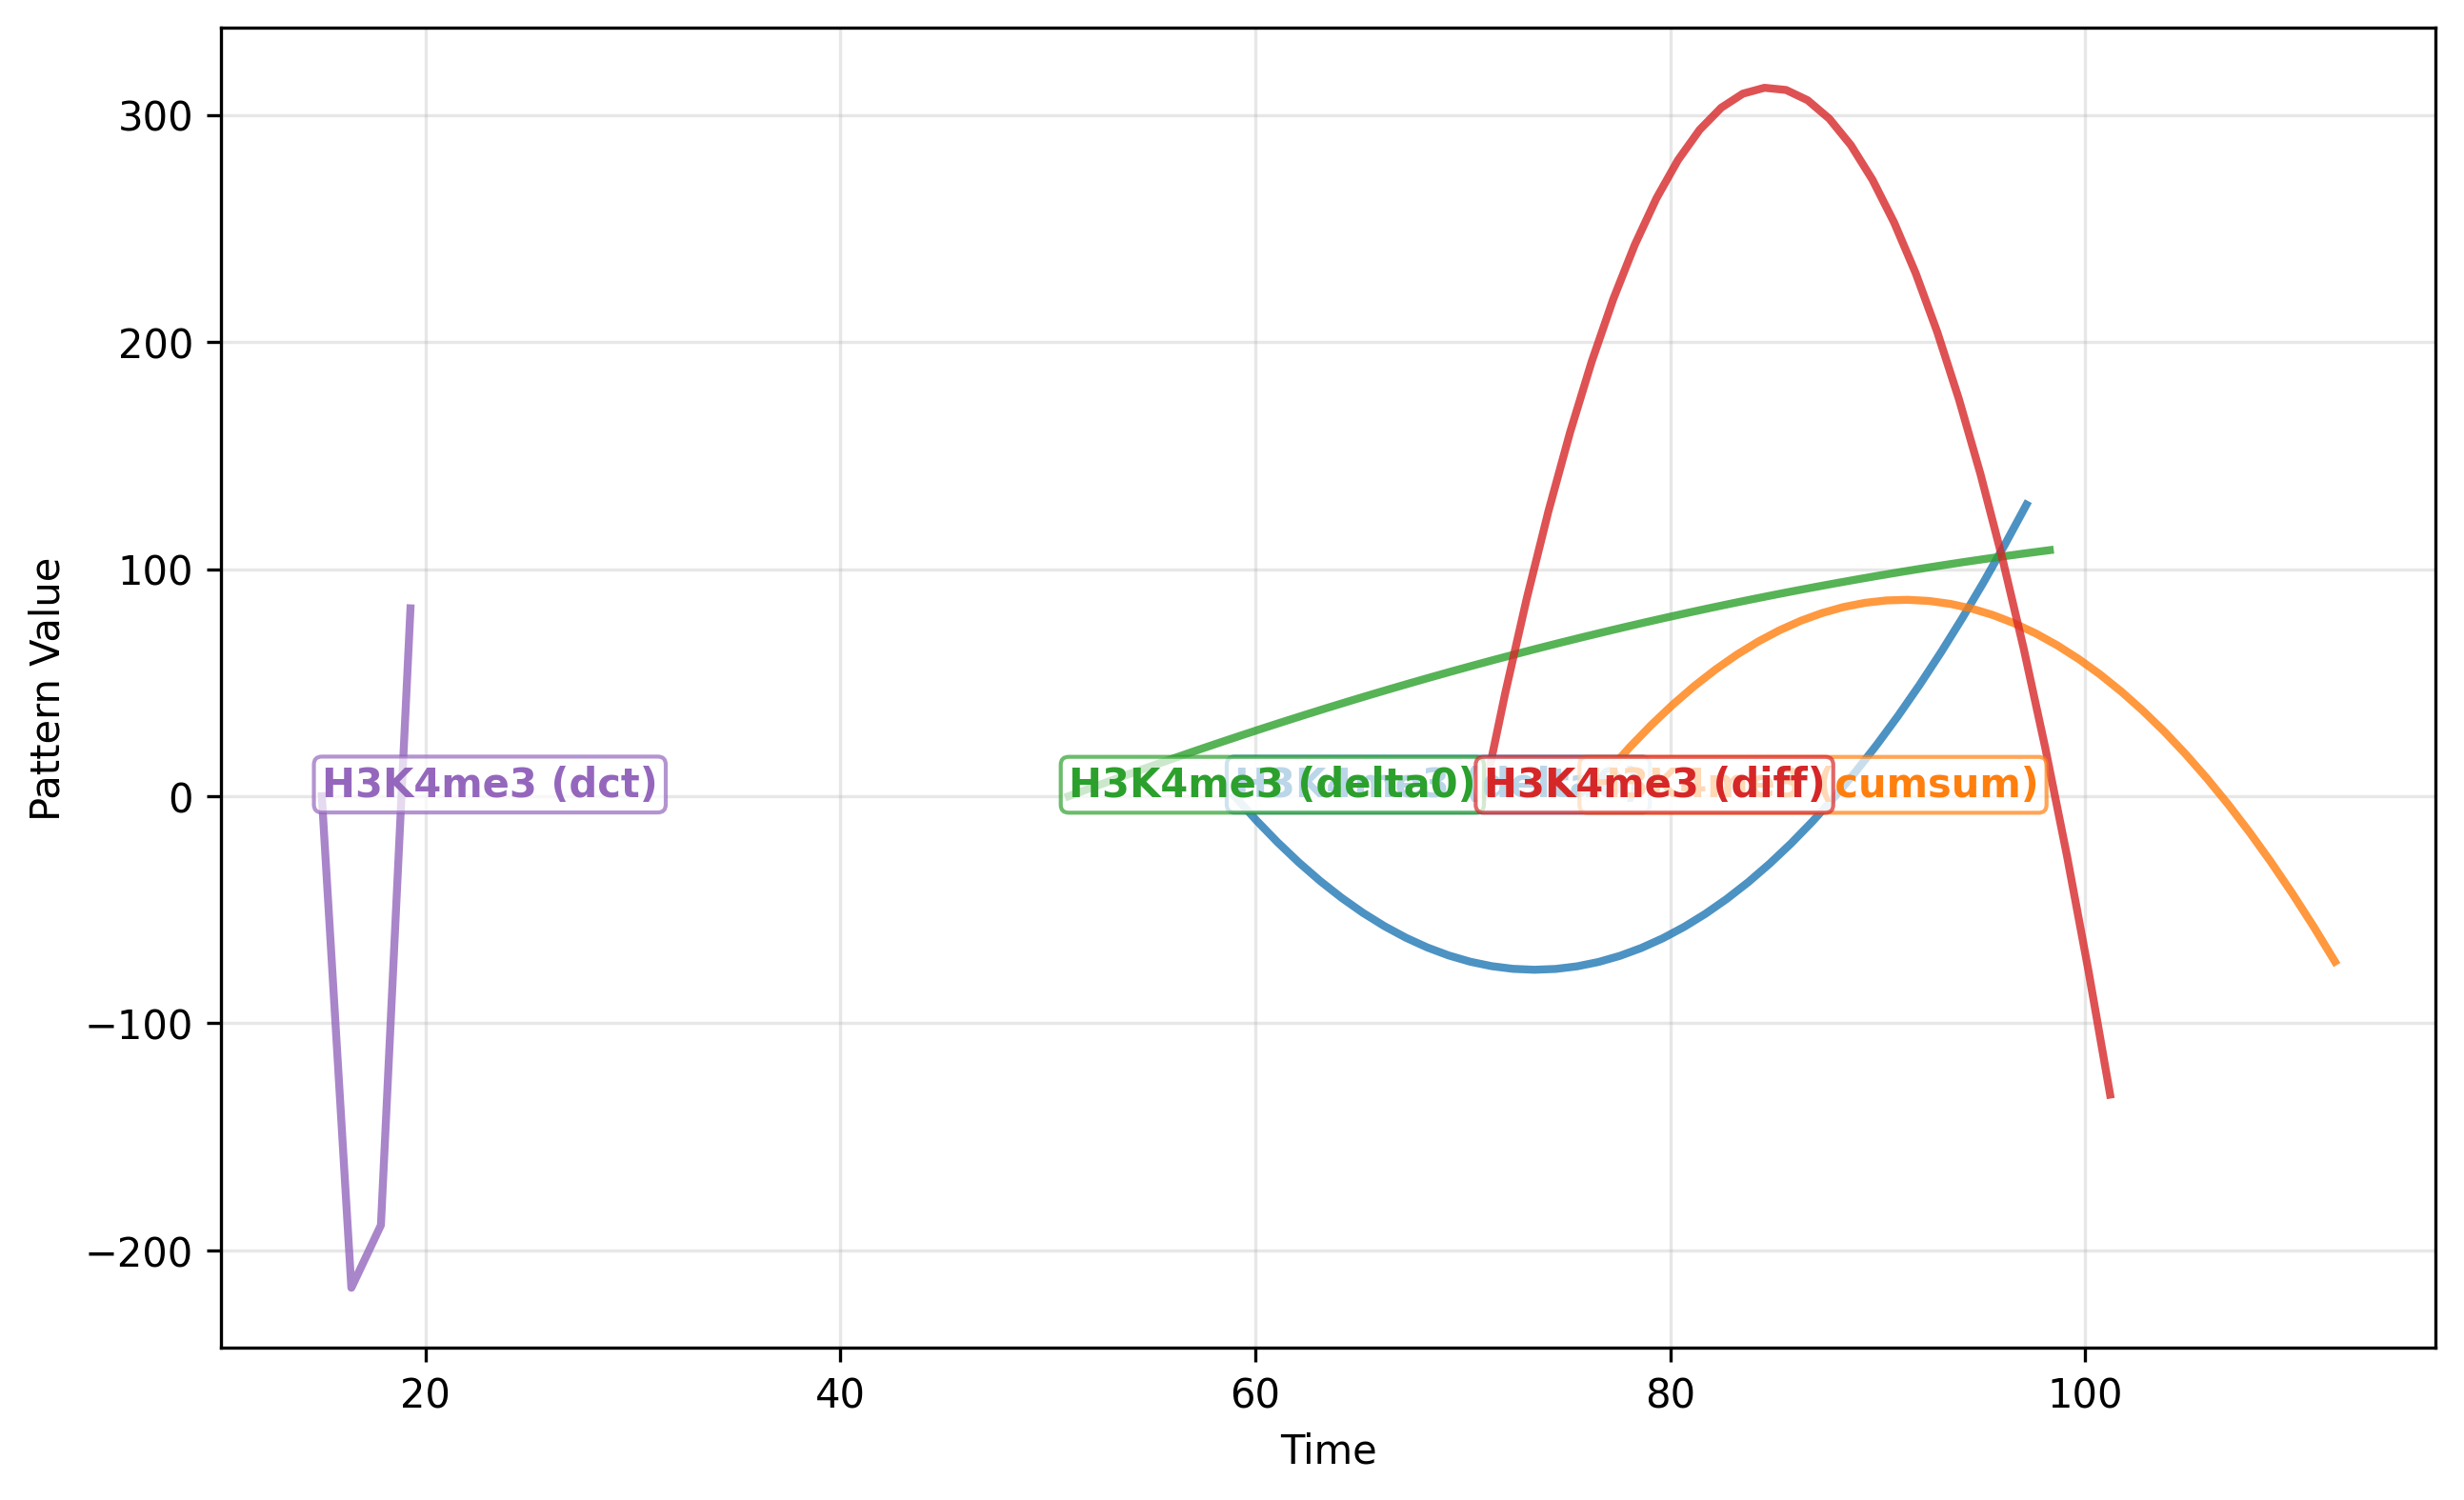
\includegraphics[width=\textwidth,keepaspectratio]
  {images/stability_remc.png}
  \caption{Pattern stability analysis for REMC (E003).
  Each colored curve represents the most important B-spline pattern discovered
  in one cross-validation fold, with annotations indicating the histone mark
  and transformation type.
  Patterns consistently target the region near the transcription start site,
  demonstrating positional stability across data splits.}
  \label{fig:pattern_stability}
\end{figure}

\section{Discussion}

The pattern search done by patX is implemented as an optimization problem over
transformation, channel, width, and search space.
To keep runtime manageable, the implementation caches transformed signals and
computes sliding-window match scores efficiently, then uses a gradient boosting
model on the resulting feature matrix.
Initial (non-pattern) features can be concatenated to the pattern features,
which is important when current context is predictive (e.g., current glucose in
forecasting tasks).
Across seven biomedical datasets, patX provides a strong accuracy--interpretability
trade-off.
It achieves the best performance on six of seven datasets while using a compact
set of pattern-based features, enabling direct inspection of what drives each
prediction.
The largest gains appear in settings where morphology and timing matter and
where clinicians benefit from interpretable, localized evidence (e.g., glucose
forecasting and ECG classification).
patX converts each sample into a small feature vector by matching a learned
template to an input signal (or transformation of that signal) and using the
resulting dissimilarity values as features.
Templates are parameterized as B-splines, which yield smooth motifs that can be
visualized and interpreted.
To reduce manual preprocessing, patX evaluates a library of candidate
transformations and retains a small subset per dataset; each pattern then
selects the transform view that best separates the labels.

The ablation study (Table~\ref{tab:ablation}) clarified which patX components
matter across domains.
On MITBIH, disabling shifting causes the largest drop (0.888 vs.\ 0.940),
supporting the need for translation-invariant matching to tolerate small
misalignments in beat morphology.
Increasing the optimization budget yields modest gains (0.944 at 1000 trials)
but increases runtime substantially, while 100 trials remains competitive.
Reducing the template to a single control point degrades performance (0.928),
indicating that non-trivial shapes are needed.

On REMC (E003), performance is comparatively stable and shifting is not required,
consistent with signals being anchored to a common coordinate frame.
On SVD, the optimization strategy has a strong effect: parallel optimization
achieves the best AUC (0.594) and improves efficiency relative to the baseline.
Overall, these results suggest that shifting and search budget should be treated
as dataset-dependent knobs rather than fixed defaults.

Interpretability in patX comes from two sources: (i) the explicit template shape
and its parameters, and (ii) the localization of where the template matches the
signal.
This enables domain experts to validate whether extracted patterns align with
known physiology (e.g., ECG wave components, histone-mark enrichment near the
TSS) and to inspect failure modes by examining which patterns activate.
In addition, feature attribution methods can be applied directly to the learned
pattern features, yielding explanations in the same units as the matching score.

\subsection{Limitations and future work}
patX trades end-to-end flexibility for transparency.
It relies on a predefined transform library and a template family, which may
miss rare or highly irregular motifs.
Runtime can be substantial when increasing the optimization budget, and the best
settings can vary across datasets, motivating automated configuration selection.
Future work includes learned or domain-specific transforms, more efficient search
strategies, richer template parameterizations, and interactive workflows that
pair pattern discovery with expert feedback.

\section{Conclusion}
We introduced patX, an interpretable pattern extraction framework bridging the
gap between handcrafted descriptors and opaque deep models through
multi-representation pattern discovery.
Through extensive experiments across seven diverse biomedical datasets, we
demonstrated that a small set of automatically discovered B--spline motifs
can provide transparent, task-specific features for standard machine learning
models, while keeping the learned representations human-readable and directly
visualizable.
The optional sliding-window matching enables translation-invariant pattern
detection, analogous to applying a convolutional filter followed by pooling,
while retaining explicit template parameters.
The B--spline representation combined with automatic transformation selection
provides smooth, locally controllable patterns that capture both shape and
amplitude information across multiple signal representations (time, frequency,
derivative domains).
Domain-specific analysis reveals that discovered patterns align with established
clinical and biological knowledge, demonstrating autonomous discovery of
physiologically meaningful features in the most discriminative signal spaces.
Future extensions will explore adaptive control point allocation, learned or
domain--specific signal transformations, semi--supervised pretraining on large
unlabeled corpora, and tighter integration with interactive visualization tools
to facilitate clinical adoption.

\bibliographystyle{elsarticle-num}
\bibliography{bibliography}

\section{Supplementary Data}

\subsection{Signal transformations and usage}
patX builds a fixed library of transformations and lets the optimizer pick the
most predictive representations. The library spans time, frequency, and
nonlinear views: raw, derivative, second derivative, cumulative sum, difference,
log1p, absolute value, sorted, DCT, exponential, tanh, sine, cosine,
reciprocal, FFT power, autocorrelation, and four wavelet bases (db4, sym4,
coif1, haar). Each transform is applied per channel to produce a parallel stack
of views of the same signals.

During training, patX first scores every transform independently using
aggregate statistics (mean, std, quantiles, skew, kurtosis, range, halves of
the series) and cross-validation, then retains the top-K transforms for pattern
search. For every candidate pattern, the optimizer selects both a transform and
channel, fits a B-spline template, and measures RMSE-based dissimilarity in the
chosen transformed space. The final model only computes features for the
selected transforms, ensuring consistency between training and inference while
keeping the search broad but the deployed pipeline compact.

\subsection{Dataset Processing Details}

\subsubsection{AZT1D Preprocessing: Insulin and Carbohydrate Response Modeling}

The AZT1D dataset presents unique challenges for glucose forecasting due to the
complex temporal dynamics of insulin and carbohydrate effects on blood glucose
levels.
Unlike simple time series where immediate effects are observed, physiological
responses involve significant delays: insulin takes 10--90 minutes to affect
glucose levels, while carbohydrates impact glucose within 10--60 minutes, with
effects persisting for 2--4 hours \cite{woldaregay2019data}.

To address these delayed physiological responses, we implement knowledge-driven
response curve modeling based on established pharmacokinetic and glycemic
response literature.
For insulin, we use a gamma-like function with 15-minute onset, 60-minute peak,
and 4-hour duration; for carbohydrates, we use 10-minute onset, 45-minute peak,
and 3-hour duration.
These response curves model the temporal dynamics of physiological effects, with
insulin effects peaking around 60 minutes and persisting for up to 4 hours,
while carbohydrate effects peak around 45 minutes and persist for up to 3 hours.

At each timepoint, we compute cumulative active effects by convolving all
historical insulin doses and carbohydrate intakes with their respective response
curves.
This creates interpretable time series that capture overlapping physiological
effects, enabling the model to understand how multiple insulin doses and meal
intakes interact over time.

The preprocessing pipeline extracts 24 timepoints (2 hours of history at
5-minute intervals) for three physiological signals: CGM values, active insulin
effects, and active carbohydrate effects.
The regression target is future glucose change $g_{t+h} - g_t$ where
$h = 30$ minutes (6 timepoints ahead).
We also include the initial CGM value (CGM\_0) as a baseline feature to provide
current glucose context.

\begin{figure}[H]
  \centering
  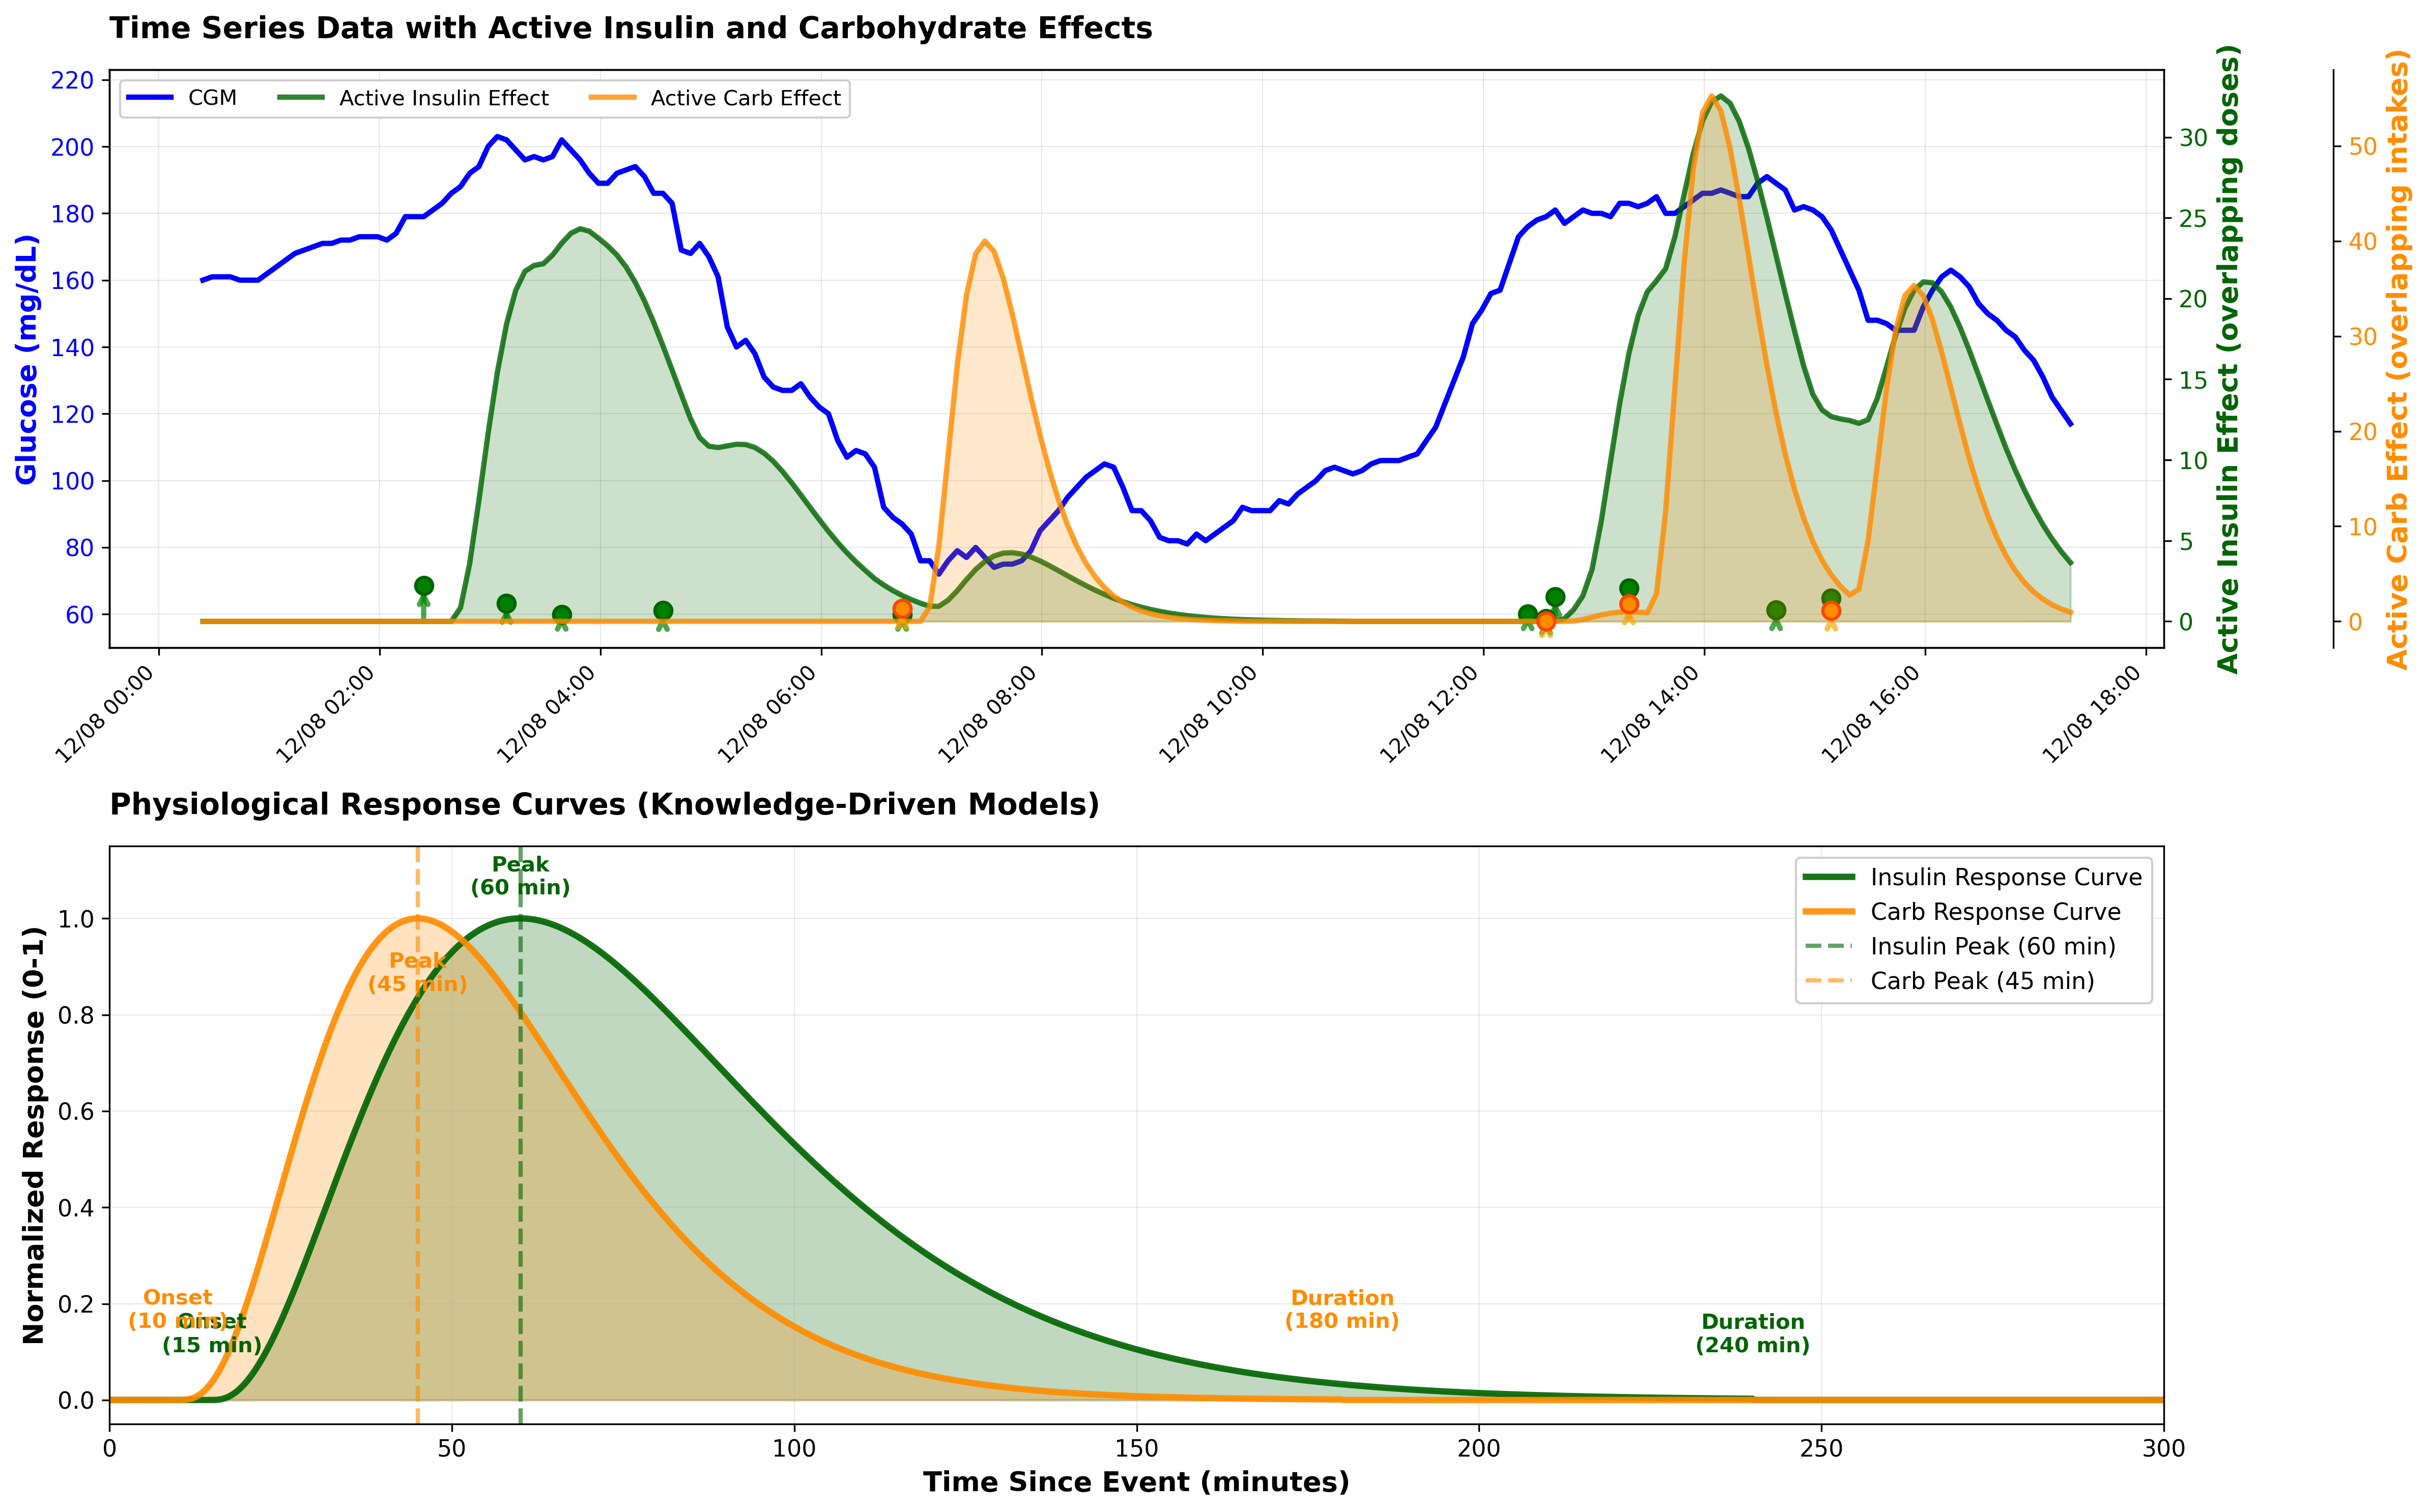
\includegraphics[width=\textwidth,keepaspectratio]
  {images/supplementary/azt1d_insulin_carb_visualization.png}
  \caption{AZT1D preprocessing visualization showing insulin and carbohydrate
  response modeling.
  Top panel: Real-time CGM with overlapping insulin and carbohydrate effects
  over time for Subject 1.
  Blue line shows CGM values with target range (70-180 mg/dL) highlighted in
  green.
  Dark green shaded area represents active insulin effect from overlapping
  doses (circles with crosses).
  Orange shaded area represents active carbohydrate effect from overlapping
  intakes (circles with crosses).
  Bottom panel: Physiological response curves showing normalized insulin
  (15-min onset, 60-min peak, 240-min duration) and carbohydrate (10-min onset,
  45-min peak, 180-min duration) effects over time.
  These knowledge-driven models enable patX to learn from physiologically
  meaningful features that capture delayed and overlapping effects.}
  \label{fig:azt1d_preprocessing}
\end{figure}

This preprocessing approach transforms raw event data into continuous
physiological signals that capture the complex temporal dynamics of glucose
regulation, providing patX with meaningful features for pattern discovery across
multiple signal representations.

\subsubsection{MITBIH Preprocessing}

The MIT-BIH Arrhythmia Database contains annotated ECG recordings from 48 patients.
We extract individual heartbeats by centering 100-sample windows around annotated
R-peak positions, with 50 samples before and 50 samples after each R-peak.
Each beat is classified into one of five arrhythmia types: Normal (N), Left bundle
branch block (L), Right bundle branch block (R), Atrial premature (A), and
Premature ventricular contraction (V).
To address class imbalance, we apply random undersampling to balance class
distributions before training.

\begin{figure}[H]
  \centering
  
\includegraphics[width=0.6\textwidth,keepaspectratio]
  {images/supplementary/mitbih_sample.png}
  \caption{Representative ECG beat from MITBIH dataset showing characteristic
  R-peak morphology.}
  \label{fig:mitbih_sample}
\end{figure}

\subsubsection{Emotions Preprocessing}

The EEG emotions dataset contains brainwave recordings collected while participants
experienced different emotional states (positive, neutral, negative).
We extract FFT-derived features from 5 EEG channels (AF3, F7, F3, FC5, T7), yielding
254 frequency bins per channel.
The FFT features are organized into two groups (a and b suffixes) representing
different frequency decomposition components, providing 5 input channels with 254
time points each for pattern discovery.

\begin{figure}[H]
  \centering
  
\includegraphics[width=0.6\textwidth,keepaspectratio]
  {images/supplementary/emotions_sample.png}
  \caption{Representative EEG frequency spectra from Emotions dataset showing
  power distributions across five channels.}
  \label{fig:emotions_sample}
\end{figure}

\subsubsection{REMC Preprocessing}

Following our prior work on PatternChrome \cite{paul2025prediction}, we predict
binary gene expression (high/low) from histone modification ChIP-seq profiles from
the Roadmap Epigenomics Consortium (56 cell lines, 19,795 genes).
We convert RefSeq to GENCODE identifiers, retaining 18,421 genes.
For each gene, we extract five histone modification signals (H3K4me1, H3K4me3,
H3K36me3, H3K9me3, H3K27me3) from 5000 bp upstream and downstream of the TSS,
divided into 50 bp bins (200 bins per mark).
Gene expression is binarized at the median level.
We split 6,600/5,911/5,910 genes for train/validation/test with balanced labels.

\begin{figure}[H]
  \centering
  
\includegraphics[width=0.6\textwidth,keepaspectratio]
  {images/supplementary/remc_sample.png}
  \caption{Representative histone modification profiles from REMC dataset showing
  all five marks (H3K4me3, H3K4me1, H3K36me3, H3K9me3, H3K27me3) around the
  transcription start site for a high-expression gene.}
  \label{fig:remc_sample}
\end{figure}

\subsubsection{MIMIC-IV Preprocessing}

We predict ARDS from multivariate clinical time series in ICU patients.
The dataset contains 29 features per subject: vital signs (respiratory rate,
heart rate, O2 saturation, blood pressure, temperature), ventilator settings
(FiO2, PEEP), Glasgow Coma Scale scores, laboratory values (arterial pH, PaO2,
creatinine, platelets, WBC, INR, lactate, bilirubin), vasopressors (norepinephrine,
phenylephrine, epinephrine, dopamine, dobutamine), urine output, and derived
features (PaO2/FiO2 ratio, pulse pressure).
We extract 24-hour time series binned hourly, with forward/backward filling for
missing values and 0.1/99.9th percentile capping for extreme values.
Subjects with $<$5 hours of data are excluded; anchor\_age is provided as baseline.

\begin{figure}[H]
  \centering
  
\includegraphics[width=0.6\textwidth,keepaspectratio]
  {images/supplementary/mimic_sample.png}
  \caption{Representative clinical time series from MIMIC-IV dataset showing
  24-hour trajectories of vital signs, laboratory values, and ventilator settings.}
  \label{fig:mimic_sample}
\end{figure}

\subsubsection{PAMAP2 Preprocessing}

The PAMAP2 dataset contains recordings from 9 subjects performing 18 physical
activities while wearing 3 IMUs (wrist, chest, ankle) and a heart rate monitor.
Each IMU records temperature, 3D acceleration ($\pm$16g and $\pm$6g scales),
3D gyroscope, 3D magnetometer, and 4D orientation at 100Hz, yielding 51 channels.
We create 100-sample windows (1 second) with 50\% overlap, filtering transient
activities (ID 0) to obtain 12 activity classes: lying, sitting, standing, walking,
running, cycling, Nordic walking, watching TV, computer work, ascending/descending
stairs, and vacuum cleaning.
Missing values are interpolated and filled with column means.

\begin{figure}[H]
  \centering
  
\includegraphics[width=0.6\textwidth,keepaspectratio]
  {images/supplementary/pamap2_sample.png}
  \caption{Representative IMU sensor data from PAMAP2 dataset showing
  acceleration and gyroscope measurements from hand, chest, and ankle sensors.}
  \label{fig:pamap2_sample}
\end{figure}

\subsubsection{SVD Preprocessing}

The Saarbr\"ucken Voice Database (SVD) contains voice recordings from over 2000
subjects, including healthy controls and patients with 71 different voice
pathologies \cite{lee2021experimental}.
Following the exact methodology of Lee \cite{lee2021experimental}, we select
balanced subsets for male and female subjects separately:
\begin{itemize}
\item \textbf{Female}: 259 healthy + 259 pathological (97 hyperfunctional
      dysphonia, 51 functional dysphonia, 30 laryngitis, 81 other)
\item \textbf{Male}: 259 healthy + 259 pathological (62 laryngitis,
      44 hyperfunctional dysphonia, 25 vocal fold polyp, 128 other)
\end{itemize}

We extract sustained vowel recordings of /a/, /i/, and /u/ at normal pitch
and apply the following preprocessing pipeline:
(1) bandpass filtering (80--4000~Hz) to remove DC offset and high-frequency
noise, (2) pre-emphasis with coefficient 0.97 to amplify higher frequencies,
(3) silence trimming using RMS-based voice activity detection,
(4) truncation to 3 seconds maximum, and
(5) resampling to 700 samples using polyphase filtering.
Each waveform is normalized to zero mean and unit variance, then clipped to
$\pm5$ standard deviations.

Following Lee \cite{lee2021experimental}, we perform separate evaluations by
gender and vowel to account for physiological differences in fundamental
frequency and vocal tract characteristics between men and women.

\begin{figure}[H]
  \centering
  
\includegraphics[width=0.6\textwidth,keepaspectratio]
  {images/supplementary/svd_sample.png}
  \caption{Representative waveforms from SVD dataset showing preprocessed
  audio signals for sustained vowels /a/, /i/, and /u/ at normal pitch.
  Each vowel is resampled to 700 samples after bandpass filtering and
  silence trimming.}
  \label{fig:svd_sample}
\end{figure}

\end{document} 